\documentclass{imc-inf}

\title{RoadGPT: AI-Based procedural generation of virtual roads}
\subtitle{}
\thesistype{Bachelor Thesis} % or Bachelor Thesis
\author{Benedikt Steininger}
\supervisor{Alessio Gambi, PhD}
\copyrightyear{2024}
\submissiondate{15.01.2024}
\keywords {Prompt Engineering, Generative AI, Autonomous Vehicles} % add keywords here

% Remove empty page after chapter  
\let\cleardoublepage\clearpage 



% \usepackage{xyz}
% ... add your own packages here!
\usepackage{listings}
\usepackage{subcaption}
\usepackage{graphicx}
\usepackage{float}
\usepackage{pdfpages}
                              

\begin{document}
\frontmatter\maketitle{}


\begin{declarations}\end{declarations}



\begin{abstract}
The emergence of self-driving vehicles marks a significant change in the automotive industry, with companies like Uber and Waymo leading the way in this new technology. To ensure road safety, it is essential to conduct rigorous testing of these vehicles, especially as they are introduced into live traffic. Field testing can be costly and risky, so most of the testing is done in simulations.

This study aimed to simplify the generation of virtual roads, which is typically reliant on domain models and heuristics. It utilized generative AI to transform textual road descriptions into detailed machine-readable formats. These outputs were then used to create roads automatically within a simulator.

The findings indicated that generative AI holds promise for this application. However, since the model used in this study was not specifically trained for this task, it encountered challenges in certain areas. These issues might be resolved by fine-tuning the current model or developing a new one.
\end{abstract}


%\begin{acknowledgements}
%This is an \textbf{optional} page. Use your choice of paragraph %style for text on this page. Usually, this space is for thanking %your supporters and getting emotional about how grateful you are %to everyone.  
%\end{acknowledgements}

\addtoToC{Table of Contents}%
\tableofcontents%
\clearpage


\addtoToC{List of Tables}%
\listoftables
\clearpage


\addtoToC{List of Figures}%
\listoffigures
\clearpage


%   MAIN MATTER  %%%%%%%%%%%%%%%%%%%%%%%%%%%%%%%%%%%%%%%%%%%%%%%%%%%%%%%%%%%%%%
\mainmatter%

\chapter{Introduction}\label{chap:introduction}


This section will discuss the research questions and the research approach of the
thesis, as well as the motivation behind it.

\section{Motivation}

Artificial intelligence (AI) has entered various industries during the past few years, including the automotive sector. From advanced driver assistance systems to Tesla's autopilot, AI is used to improve traffic safety. Testing autonomous vehicles in actual traffic situations would be risky, defeating the goal of assuring safety.

As a result, simulations are used to test autonomous vehicles. These simulations are created by generating roads and environments to analyse the cars' behavior. Most existing approaches for road generation rely on domain models and metaheuristics. They are limited to generating 2D roads with fixed layouts. These problems could be solved using generative AI.

Generative AI is a branch of Artificial Intelligence that focuses on creating new content. With the use of large language models like ChatGPT \cite{ChatGPT}, there is potential to generate virtual roads for testing by providing verbal descriptions such as "mountain road" or "highway". The output of ChatGPT can then be automatically translated and passed into driving simulators.

\section{Research Questions}
The primary objective of this thesis is to answer the following research question.

Research Question 1 (RQ1): Can generative AI be used to automatically create three-dimensional roads for testing autonomous vehicles?

By harnessing the capabilities of generative AI, the tool streamlines the process of generating roads for self-driving vehicles, eliminating the necessity for complex algorithmic coding.


\section{Research Method}
The research approach consists of four main phases: a review of the state-of-the-art project, implementation of the project, and data gathering and analysis of the data. The findings of the state-of-the-art will serve as a basis for the implementation of the project.

The implementation can be divided into four parts that build on each other. The first part consists of prompt engineering (see section \ref{prompt engineering}) and receiving the output in a format that can be used in the next part. In the second part, a Python script will translate the output into road nodes and interpolate the road. The third part consists of validating the correctness of the road (steepness, sharpness of turns, etc.). The fourth part is building the road in the simulator. The roads will then be evaluated in the context of a user study. 

The quantitative data gathered through the validation script and the user study will then be used for a statistical analysis of the results.

\begin{figure}[ht!]
	\centering
	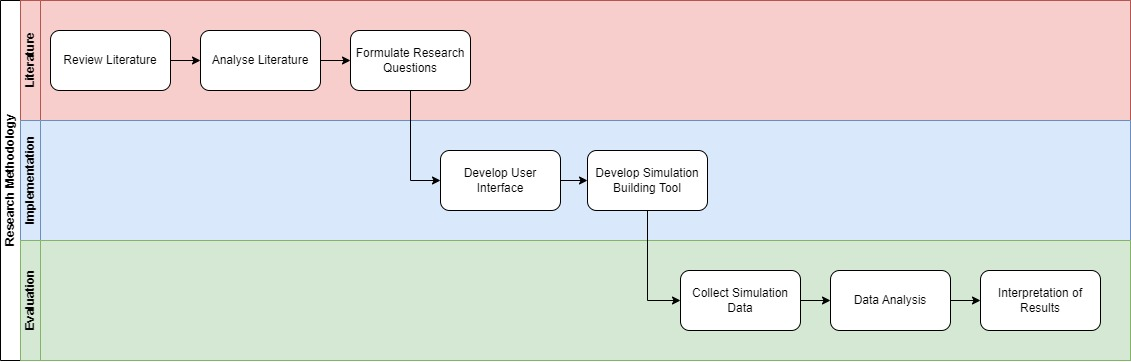
\includegraphics[width=1\linewidth]{images/Research_Methodology.jpg}
	\caption{Research Methodology \label{research methodology}}
\end{figure}

\section{Structure}
The bachelor thesis is structured as follows:
\begin{itemize}
	\item Chapter 1: Introduction

 
    The opening chapter of this bachelor thesis holds significant importance in setting the stage for the research. Within this section, I provide a thorough outline of the motivation driving the study, articulate the fundamental research questions, and present a concise overview of the chosen research methodology. By elaborating on the motivation, the significance and relevance of the study in a broader context is established. The formulation of research questions provides a clear roadmap, guiding readers through the central inquiries shaping the investigation. Furthermore, a comprehensive discussion of the selected research methodology offers insights into the tools and approaches used to address the research questions. This chapter serves as an essential guide, laying the foundation for subsequent chapters and contributing to the overall coherence and clarity of the thesis.
	
	\item Chapter 2: Background
	
	This chapter provides a thorough background that explains the domains and technologies related to the topic. Its primary objective is to supply readers with an overview and the essential vocabulary necessary for understanding the following chapters. By exploring relevant domains, this section seeks to place the research within a broader context, providing the foundation of the study. Additionally, an examination of related technologies is conducted to acquaint the reader with the tools and methodologies essential to this research.
	
	\item Chapter 3: Related Work
	
	The "Related Work" chapter forms a critical component of this bachelor thesis, offering a comprehensive analysis of existing literature and research relevant to the subject matter. In this section, a thorough review of the current state of the art within the field is conducted, examining scholarly contributions, methodologies, and findings that are directly connected to the research objectives. By critically evaluating the existing body of work, gaps, trends, and debates in the literature can be identified. This structured examination of the related work is crucial for establishing the academic foundation of the thesis and demonstrating the unique contributions of the research.
	
	\item Chapter 4: Methodology
	
	This chapter provides a comprehensive overview of the methodology used in this thesis. It offers detailed insights into the systematic approach taken to address the research questions. The chapter covers the research design, data collection methods, and analytical techniques employed, aiming to bring clarity to the procedural aspects of the study. By outlining the methodology, this section not only serves as a guide for potential replication but also establishes the credibility and robustness of the research, laying a solid foundation for the subsequent analysis and interpretation of findings.

    \item Chapter 5: Implementation
    
    Chapter 5 focuses on the practical implementation of the project, explaining how the code works and which technologies were used. It provides a detailed explanation of the project's technical aspects, including the software tools and programming language utilized. This chapter aims to offer readers a clear understanding of how the project was implemented.

    \item Chapter 6: Evaluation
    
    The "Evaluation" chapter serves as a comprehensive exploration of the methods used for assessing the tool's effectiveness. It extensively discusses the procedures used for data collection, analysis, and interpretation. Additionally, it provides a detailed exploration of the user study used to evaluate the tool, covering its setup and execution. Through a thorough examination of these elements, the chapter aims to offer a comprehensive understanding of the evaluation process and provide insights into the tool's performance.
	
	\item Chapter 7: Summary
	
	This chapter presents the main findings of the study. The insights obtained from the results are presented by systematically analyzing and interpreting the collected data. The findings are discussed in detail, highlighting their relevance to the research questions and objectives.
\end{itemize}
\chapter{Background}
In this section, the background of the most important technologies used will be presented, setting up grounds for discussion.

\section{Artificial Intelligence}

IBM defines Artificial Intelligence as the use of technology to enable computers and machines to replicate human intelligence and problem-solving abilities.

Artificial intelligence (AI), whether used independently or combined with other technologies like sensors and robotics, accomplishes tasks that are typically performed by humans. Examples include digital assistants, GPS navigation, autonomous vehicles, and sophisticated AI tools like OpenAI's ChatGPT, which are widely used in today's society.

In the field of computer science, AI includes areas like machine learning and deep learning, which aim to mimic human thinking through algorithmic systems. These algorithms can "learn" from the data they receive, getting better at making decisions over time through continuous improvement processes.


Artificial intelligence can be categorized into two groups: Weak AI and Strong AI.

Weak AI, also called narrow AI or artificial narrow intelligence (ANI), is designed and trained for specific tasks, driving much of today's AI applications like Siri, Alexa, IBM Watson, and self-driving cars. On the other hand, strong AI consists of artificial general intelligence (AGI) and artificial super intelligence (ASI). AGI aims to match human intelligence, possessing self-awareness and problem-solving abilities, while ASI would surpass human intelligence. Although strong AI remains theoretical, ongoing research explores its potential \cite{IBM}. 

\subsection{Natural Language Processing}

Natural Language Processing (NLP) refers to a set of computational techniques designed for automatically analyzing and representing human languages. It involves tasks such as accessing and acquiring lexical, semantic, and episodic characteristics of language, creating and propagating dynamic bindings, manipulating recursive structures, coordinating processing modules, identifying language constructs, and representing abstract concepts. The ultimate goal of NLP is to advance from basic language processing to achieving natural language understanding, which involves grasping context and meaning beyond mere syntactic structures. Presently, NLP heavily relies on syntactic representations, which are constrained by their inability to incorporate background knowledge similar to human comprehension. The focus of NLP centers on replicating human cognitive processes and leveraging semantic features that are implicit in the text. These computational models support both theoretical exploration and practical implementations, enabling efficient communication between humans and machines \cite{Chowdhary2020}.

\subsection{Transformers}
Transformer architectures leverage a self-attention mechanism to understand relationships within sequences, allowing them to capture long-range dependencies more effectively compared to recurrent networks. Unlike traditional models that rely on recursion, Transformers process entire sequences at once, improving scalability and efficiency. They are built solely on attention mechanisms, with a unique implementation known as multi-head attention, optimized for parallelization. Transformers excel in handling complex models and large datasets, offering advantages over alternatives like hard attention, which relies on stochastic sampling. Due to their minimal prior knowledge assumption, Transformers are typically pre-trained on large-scale unlabeled datasets using pretext tasks, enabling them to encode rich and generalizable representations. These representations are then fine-tuned on supervised tasks to achieve optimal performance \cite{KhanNHZKS}.

\subsection{Generative and Conversational AI}

Generative AI is a type of Artificial Intelligence that uses deep learning models to create human-like content in response to complex prompts, such as languages, instructions, or questions. Examples of this technology include OpenAI’s ChatGPT \cite{ChatGPT} and DALL-E \cite{DallE}. These AI models generate responses that go beyond their explicit programming, distinguishing them from other AI models. Conversational AI is an Artificial Intelligence subset that focuses on human-like interactions, often relying on predefined responses. However, some Conversational AI models can also generate content. Models like ChatGPT use both Generative and Conversational AI to enhance their capabilities, allowing them to better simulate human conversation and generate more dynamic responses. \cite{LimGPPP}

\subsubsection{ChatGPT}
ChatGPT, an AI-driven service accessible online, is designed for tasks such as text organization, summarization, and composition. GPT, short for "Generative Pre-trained Transformer", describes the manner in which ChatGPT processes requests and generates responses. It is built to understand and respond to user queries and commands by analyzing extensive text data to grasp word relationships. By predicting the most probable next word, similar to search engine auto-complete features, ChatGPT refines its responses iteratively. During training, exemplified by completing sentences such as "instead of turning left, she turned ...", ChatGPT evolves from random word suggestions to more accurate predictions. Because of the wide variety of possible answers, the model's numerical settings, called "weights" or "parameters," slowly change as it learns, capturing what it learns without saving or copying the original sentences \cite{OpenAICGPT}.

In response to natural language inputs, also called "prompts", ChatGPT provides text output. One example of such a prompt would be: "Explain to me in one paragraph what ChatGPT is." ChatGPT provided the following answer (Fig \ref{ChatGPT}).

\textit{
	ChatGPT is an advanced language model developed by OpenAI that uses deep learning techniques to generate human-like text responses. Trained on a vast amount of internet text, it has the ability to understand and generate coherent and contextually relevant responses to user queries, making it a powerful tool for conversational interactions, information retrieval, and providing assistance across a wide range of topics.} \cite{OpenAI} 

\begin{figure}[ht!]
	\centering
	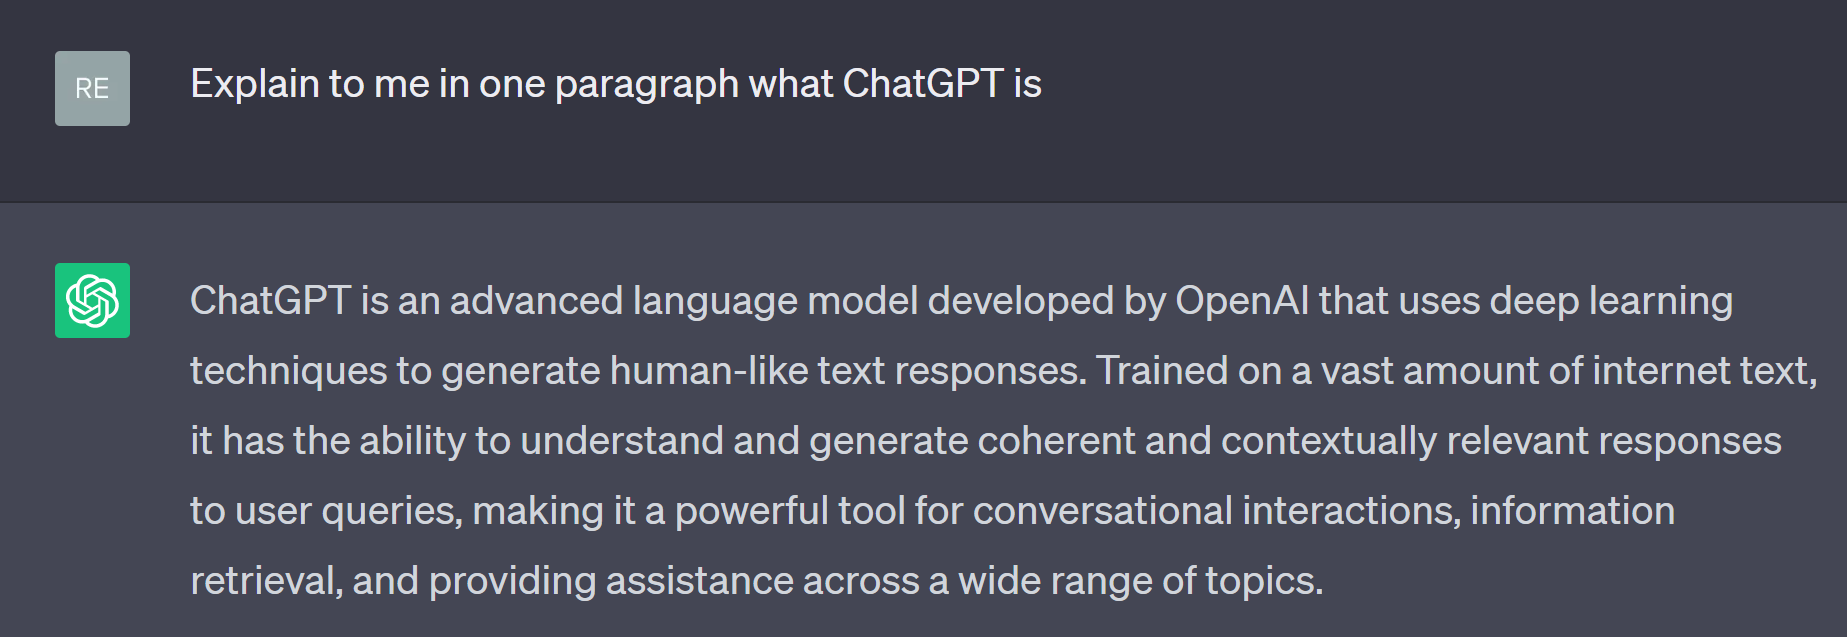
\includegraphics[width=90mm]{images/ChatGPT.png}
	\caption{ChatGPT - prompt and answer \label{ChatGPT}}
\end{figure}



\subsubsection{Prompt Engineering}
\label{prompt engineering}
Prompt engineering is the process of using prompts to program Large Language.
Models (LLMs), like ChatGPT. An LLM is given a set of instructions called a prompt
to help it tailor its output and user interactions. Engineering prompts to enforce
rules, automate procedures, and guarantee particular output qualities and output
quantities, which is known as prompt engineering. It is an ever-more-important skill set
required to communicate with LLMs and can be used to address a variety of issues,
such as automating software development tasks when speaking with LLMs. \cite{WhiteFHSOGESS}

Microsoft outlined a set of best practices in their guide to prompt engineering.

\begin{itemize}
	\item \textbf{Be specific}: Provide clear and precise instructions, minimizing room for interpretation and narrowing the operational scope.
	
	\item \textbf{Be descriptive}: Use descriptive language and analogies to enhance understanding.
	
	\item \textbf{Double Down}: Reinforce key points by repeating instructions, both before and after presenting primary content, employing cues for better comprehension.
	
	\item \textbf{Order Matters}:  Consider the order of information presentation, as it can influence the model's output. Be mindful of whether instructions precede or follow content, and recognize the impact of recency bias in the order of few-shot examples.
	
	\item \textbf{Give the model an "out"}: Offer the model an alternative option or an "out" in case it struggles with the assigned task. For instance, suggest a default response like "not found" to help the model avoid generating inaccurate information.\cite{MicrosoftLearn}
	
\end{itemize}

\section{Autonomous Vehicles}
There are six levels of driving automation, ranging from no driving automation (Level 0) to full driving automation (Level 5). At Level 0, vehicles are entirely manually controlled, with no automation in the dynamic driving task. 

Level 1 involves a single automation feature, like cruise control or steering assistance, while the driver retains control over other driving tasks. At Level 2, the car takes control over steering, acceleration, and braking. However, it still requires supervision from a human driver, who must take control when necessary.

Level 3 marks conditional driving automation, in which vehicles have environmental detection capabilities and can make informed decisions. However, human supervision and intervention are still necessary.

Level 4 introduces high driving automation, allowing vehicles to intervene in the event of system failures. While these cars can operate in self-driving mode, their use is limited to specific areas.

Level 5 represents full driving automation, where vehicles no longer require human attention. These fully autonomous cars have the ability to operate without restrictions, mimicking the capabilities of experienced human drivers.

Autonomous vehicles are vehicles that operate on Level 5 of the driving automation levels, which means they do not require human interaction\cite{Synopsys}\cite{SAEMobilus}\cite{TWI}.



\section{Computer Simulation}
The Cambridge Dictionary defines a simulation as \textit{a model of a real activity, created for training purposes or to solve a problem} \cite{CambridgeSim}.

A computer simulation is a program that imitates the operations of a real-world system or process over time. This program, referred to as a computer simulation model, uses algorithms to calculate the system's states over a specified time period, effectively creating a numerical representation of the system's evolution. The simulation generates data that can be visualized, often in a manner resembling scientific instrument readings. Simulations are typically used when a model's mathematical equations are complex and cannot be solved analytically, necessitating step-by-step computational methods. It's worth noting that the term "computer simulation", in the narrowest sense, refers to a specific implementation of an algorithm on a particular digital computer using a specific language and compiler. Variations in these elements can result in different outcomes from the simulation \cite{Winsberg}.

\subsection{Beamng.tech}
BeamNG.tech is an adapted version of the simulation game BeamNG.drive, created for academic and industrial purposes. While sharing many similarities, BeamNG.tech extends its functionality to support driver training and advanced driver-assistance systems (ADAS). It utilizes a soft-body physics engine for vehicle simulation \cite{BeamNG}.

Soft-body physics, as implemented in BeamNG.drive, is a fundamental aspect of the game's physics model. Unlike traditional "Rigid Body" physics simulation found in most games, BeamNG.drive utilizes a "Soft Body" physics simulation, which means that objects such as cars are deformable, allowing for more realistic and dynamic interactions \cite{BeamNGphysics}.

Additionally, BeamNG.tech incorporates tools such as BeamNGpy, a Python interface that automates testing and data gathering. Although its primary focus is on simulating ground-based vehicles, BeamNG.tech also offers simulations for air and maritime scenarios. Its research-oriented features include a sensor suite equipped with cameras, LIDAR, ultrasonic, electric, and IMU sensors tailored specifically for autonomous driving applications. BeamNGpy streamlines testing scenarios for learning systems and ensures the validation of autonomous driving software. While BeamNG.tech is not open-source, researchers can apply for a free license on their website \cite{BeamNG}.

\section{Procedural content generation}
In the realm of video games, procedural content generation (PCG) is the practice of using algorithms instead of manual design to generate elements like levels, characters, or environments. PCG has become increasingly significant in game development and technical game research because of its ability to efficiently create diverse and dynamic content. This approach involves the methodical application of algorithms and rules to produce content, providing developers with an automated and adaptable method to create a wide range of unique gaming experiences \cite{GambiMMFG}\cite{SummervilleSGHHINT}.

Procedural generation in the context of virtual roads involves generating roads by seamlessly connecting individual road segments. This approach ensures a continuous and gapless network, where each segment's front line serves as the back line for the subsequent one, resulting in a smooth transition. The procedural generation process also ensures that roads with impossible configurations are not created in order to maintain validity \cite{GambiMF}\cite{GambiMMFG}. 

\section {Testing of autonomous vehicles}

Testing is essential to make sure autonomous vehicles are safe, dependable, and compliant with the law. It helps to reduce risks and improve algorithms for making
decisions. Such testing increases public confidence in the technology by demonstrating safe and efficient functionality in a variety of driving scenarios.

\subsection{Field Testing}
Autonomous vehicles can be tested in real-world scenarios, like Google driverless cars, which are tested mainly in real traffic, according to Huang et al. \cite{HuangKYF}. Other real-world testing approaches include testing facilities. This form of testing is particularly beneficial because it mirrors the environment where the autonomous vehicle will eventually operate, providing a realistic assessment of its performance. 

While tests in real-world settings are always the final step in the validation chain, according to Huang et al., self-driving cars would have to drive hundreds of millions of kilometers without accidents to prove their safety statistically \cite{HuangKYF}. Since that is not feasible because of time and cost, simulation-based testing offers an alternative \cite{SchoenerHP}.

\subsection{Simulation-based testing}
The simulation-based testing of autonomous cars is carried out in a virtual setting, where the vehicles are evaluated against a variety of simulated scenarios that resemble real-world events. These scenarios can be repeated and altered as many times as necessary, incorporating different weather conditions, pedestrian movements, and traffic conditions. This allows the testing of uncommon or risky events without any real risk. Simulation testing is very valuable because it enables thorough testing in less time and at a lower cost than real-world testing. However, there are limitations since it depends on how accurately the simulations capture the complexity and unpredictability of real-world driving \cite{GambiMF}\cite{HuangKYF}\cite{PathrudkarMSC}.

\section{Context in Domain}
In the practical implementation, the prompts provided to ChatGPT will consist of high-level descriptions of roads. ChatGPT will generate more detailed descriptions of those roads as output. Subsequently, a Python program will translate these detailed road descriptions into nodes containing x, y, and z-coordinates. These translated road nodes will then be passed into the simulator using the BeamNGpy library. Within the simulator, a scenario will be constructed based on the road nodes received from the Python code, allowing for the visualization and simulation of the generated roads. By combining ChatGPT’s language generation capabilities, Python programming, and the simulation environment provided by BeamNG.tech, this system enables the generation, translation, and simulation of roads based on textual descriptions.
\chapter{Related Work}
In this chapter, related works will be discussed.

\section{Generation of Virtual Roads}
Gambi et al. point out that the conventional methods of testing autonomous vehicles in actual traffic situations pose significant risks, are expensive, and have resulted in fatal incidents. In response to these challenges, the authors devised a solution known as AsFault. This automated tool tests software for self-driving cars by creating virtual road networks and simulating driving scenarios. It utilizes a combination of a genetic algorithm and procedural content generation to create road networks that expose potential safety issues. The primary objective is identifying bugs and problematic environmental conditions that can cause self-driving cars to fail. AsFault focuses explicitly on testing the software's lane-keeping capability. By evolving the road networks based on a fitness function that considers the distance between the car and the center of the lane, AsFault generates test cases where the car deviates from its intended path. The tool can be installed as a Python package and relies on the BeamNG.research driving simulator. Test cases generated by AsFault are saved in JSON format and can be re-executed. It also provides visualizations of the results, including the number of instances where the car goes out of bounds and the coverage of road segments achieved by the generated test suite \cite{GambiMF}.

In their research, Tang et al. showed that High-definition (HD) maps, which are critical for evaluating ADSs in simulated environments, come with certain limitations. They include features such as road networks, traffic lights, and signs, which essentially influence the range of testing scenarios, directly affecting the tests' effectiveness. However, several issues arise with these HD maps. Firstly, commercial HD maps often have a significant quantity of repeated elements, such as junctions of similar shapes, leading to a lack of diversity in the testing scenarios. Secondly, the HD maps included with open-source simulators are usually relatively small, possessing a restricted number of roads and junctions, further limiting the diversity of testing scenarios. Thirdly, the unique junction structures found in different cities or regions make it time-consuming to test ADSs thoroughly across various HD maps from different locations. Lastly, the process of manually creating diverse HD maps using specific tools is quite demanding and labor-intensive, especially considering the myriad of scenario requirements \cite{TangZYZRLZC}.

To address these issues, Tang et al. introduced an innovative solution called Feat2Map. This is an automated framework for generating HD maps based on essential features, tailored for simulation testing of autonomous driving systems. It operates by taking existing maps, extracting crucial features, and then utilizing combinatorial sampling to generate grid-layout HD maps. Feat2Map is also designed to accept manual feature configurations, providing a degree of customization flexibility. The goal of this framework is to eradicate duplicated intersections, while also ensuring a maximum diversity of intersection structures and potential scenarios. The end result is a concise HD map that maintains a comparable level of scenario diversity \cite{TangZYZRLZC}.

The Search-Based and Fuzz Testing (SBFT) workshop, previously focused on Search-Based Software Testing (SBST), aims to bring together researchers and practitioners from SBST, Fuzzing, and Software Engineering to discuss and advance the automation of software testing. The workshop aims to explore the application of search and fuzzing techniques in testing, as well as their integration with other software engineering areas. The workshop includes a research track, keynotes, testing tool competitions, and a panel discussion to facilitate knowledge sharing and foster new advancements in SBFT research \cite{SBFT}.

One of the competitions inside the SBFT workshop is the CPS (Cyber-Physical Systems) Testing Tool Competition, which aims to encourage researchers to investigate the problem of testing safety-critical CPSs (such as self-driving cars) and provide a shared framework for benchmarking test generators. The competition involves generating the highest number of diverse failure-inducing inputs, i.e., valid virtual roads that cause the autonomous vehicle to drive out of the lane. The infrastructure detects a failure each time the ego-car (partially) drives outside the lane, and the competitors are ranked based on various aspects of test generation, including their ability to generate valid test cases and trigger out-of-bounds episodes \cite{GambiJRZ}.

Pathrudkar et al. introduced the SceVar (Scenario Variations) database to enhance the realism of simulations. This database improves autonomous vehicle testing by generating realistic variations of scenarios based on real-world driving data. These variations enable a wide range of scenarios for simulation-based regression testing. The SceVar database significantly advances autonomous vehicle testing by incorporating key features such as semantic data models, real-world statistical analysis, statistical insights, and smart scenario variations. Leveraging semantic data models, it comprehensively represents static and dynamic entities in the road-traffic ecosystem, fostering intuitive interactions. Through the analysis of real-world driving data, the database extracts authentic traffic patterns, enabling the creation of numerous realistic scenario variations for simulation-based testing. The integration of statistical analysis allows for insights, pattern identification, and a focused reduction of the simulation state space. Moreover, the database facilitates the creation of smart scenario variations based on statistical insights, covering a wide range of test cases while minimizing the number of simulation runs. Collectively, these features contribute to the efficiency, accuracy, and cost-effectiveness of autonomous vehicle testing in simulation-based environments \cite{PathrudkarMSC}.
\chapter{Methodology}
The research methodology carried out in this study is depicted in Fig. \ref{research methodology}. This chapter will further discuss the implementation and evaluation of the thesis.

\section{Methods}
In terms of practical application, a Python script was implemented that accepts user input and transfers it to ChatGPT. The response from ChatGPT will then be transformed into road nodes, which will subsequently undergo interpolation processes. Following this, the program will evaluate the validity of the designed road, ensuring they do not contain overly steep gradients or excessively sharp turns and do not overlap. If the road is validated successfully, it will be integrated into BeamNG.tech, a physics-based vehicle simulation environment. The roads were then evaluated in a user study to identify whether they aligned with the description specified by the initial user input.

\section{Implementation}
A collection of Python libraries was used to implement this project. The OpenAI library enabled communication with ChatGPT, which is essential for user-AI model interaction. The BeamNGpy library was used to construct detailed road simulations. The task of interpolating road nodes is handled by the NumPy and SciPy libraries, which are renowned for their superior mathematical and scientific computation capabilities. As I built this program, I drew inspiration from the tool AsFault \cite{GambiMF}, as well as the methodologies from SBFT’s Cyber-Physical Systems (CPS) testing competition \cite{SBFT}. This integrated and inspired approach will help ensure an efficient, thorough implementation and analysis of the resulting roads.

\section{Evaluation}
For the evaluation of the project, I gathered data corresponding to the generated roads and conducted a statistical analysis to determine the extent to which they meet the specified requirements. This data collection involved assessing multiple factors such as:

\begin{itemize}
	\item validity of the road
	\item alignment between the generated road and the given prompt
	\item diversity of generated outputs using identical or similar prompts
\end{itemize}

The assessment of output validity was systematically acquired during the generation of the roads through an implemented script. Quantitative data regarding the alignment between the generated output and the given prompt, as well as the diversity of the generated outputs, was collected through a user study.

By evaluating these parameters, I was able to quantify the proportion of roads that fulfill the given requirements versus those that do not. The chi-squared test, as explained in \ref{chi-squared}, was used to determine whether there is a statistically significant difference in the number of valid roads generated as the prompts become more detailed. 
Furthermore, to assess the performance of ChatGPT in generating road descriptions, I will analyze how frequently it produces identical or similar roads when provided with vague descriptions. This analysis will shed light on the model’s ability to generate diverse and contextually appropriate road-related responses.

\subsection{Chi-Squared Test} \label{chi-squared}
The chi-square test is a statistical method used to determine whether there is a significant association between two categorical variables. It assesses whether the observed distribution of categories for one variable differs from what would be expected if the two variables were independent \cite{Freedman_2007}.

To conduct a chi-square test, categorical data is organized into a contingency table, with rows representing one variable and columns representing the other. The observed frequencies of categories in the table are then compared to the expected frequencies, which are calculated based on the assumption of independence between the variables \cite{Freedman_2007}.

The test statistic is computed by summing the squared differences between observed and expected frequencies, divided by the expected frequencies \cite{Freedman_2007}. 

The dimensions of the contingency table determine the degrees of freedom for the chi-square test. Once the test statistic is calculated, its significance level (p-value) is assessed. If the computed chi-square statistic is greater than a critical value at a chosen significance level, the null hypothesis of independence is rejected, suggesting a significant relationship between the variables. On the other hand, if the computed statistic does not exceed the critical value, the null hypothesis is accepted \cite{Freedman_2007}.

\chapter{Implementation}
This section covers the implementation of the tool, the technologies used, and the code's organization. It also outlines the tool's purpose and its target users.

\section{Purpose and Intended Audience}
The tool targets researchers and developers involved in testing self-driving vehicles. Its purpose is to streamline road creation for testing these cars, eliminating the need for users to write road generation algorithms. Instead, they can simply provide textual descriptions of the roads they want to create.


\section{Technologies}
\subsection{Python}
RoadGPT is written in Python, an \textit{"interpreted, object-oriented, high-level programming language with dynamic semantics"} \cite{python}. Python enables rapid development across different domains, from web development to data analysis and machine learning. With its extensive standard library and numerous third-party packages, it helps programmers solve complex problems efficiently \cite{python}. The main libraries used for the tool are the following:

\begin{itemize}
    \item \textbf{OpenAI}: provides easy access to the OpenAI API and is used to communicate with ChatGPT \cite{OpenAI}.
    \item \textbf{NumPy}: an open-source library used for working with numerical data in Python. It includes a wide variety of mathematical functions \cite{NumPy}.
    \item \textbf{SciPy}: a collection of mathematical algorithms and functions built on NumPy \cite{SciPy}.
    \item \textbf{BeamNGpy}: a package that provides a Python API to BeamNG.tech \cite{BeamNGpy}.
\end{itemize}

\subsection{OpenAI API}
The OpenAI API is used to enhance user road descriptions by returning more detailed descriptions in a standardized format, simplifying further processing. I selected the GPT-3.5 turbo model for this task because it supports enforced JSON responses. At the time of writing, the model is priced at \$0.0005 per 1000 tokens for inputs and \$0.0015 per 1000 tokens for outputs. Tokens represent pieces of words, with 1000 tokens approximately equaling 750 words \cite{OpenAIPricing}.

\subsection{BeamNG.tech}
BeamNG.tech has been chosen as the simulator for several reasons. Firstly, the BeamNGpy package simplifies scenario creation and data extraction for visualization. Secondly, the use of mesh roads enables the generation of 3D roads. Lastly, BeamNG.tech features a realistic physics simulation, ensuring accurate vehicle behavior and environmental interactions. Together, these attributes make BeamNG.tech a comprehensive and reliable option for simulation tasks.

%\section{Code Structure}
%Since the code is based on the SBST tool competition \cite{GambiJRZ} the code follows a similar structure. The \textbf{levels\_template/tig folder}, contains the files to create the level, alongside the textures of the roads.

%In \textbf{self\_driving} you can find the files related the simulations in BeamNG.tech. The files in this folder are used to set up and run the simulations.

%The files in the \textbf{code\_pipeline} folder 



\section{RoadGPT}
RoadGPT is a command line tool that can be called with different parameters. The code is based on the SBFT tool competition \cite{SBFT}.

\begin{itemize}
    \item \textbf{beamng-home}: The location of the BeamNG.tech executable.
    \item \textbf{beamng-user}: A directory where levels and other BeamNG-related data will be copied
    \item \textbf{model}: A parameter specifying whether to use OpenAI's assistants or the completions API. Assistants use instructions to tune their personalities and capabilities \cite{OpenAI}. Once created, users can access existing assistants by the latter's ID. Completion models take a list of messages as input and return an answer generated by the model \cite{OpenAI}. In the case of RoadGPT, these messages are just the system message, giving the model some context, ground rules, and the user's road description.
\end{itemize}

\subsection{OpenAI API Connection}
After the user provides the road description and specifies the generation budget (the number of road descriptions to be obtained from ChatGPT), RoadGPT initiates an API call using the provided parameters. This API call includes a system prompt, a prompt specified by the user, and defines the response format as JSON. The system prompt serves as the initial instruction for the model, guiding it on what to generate based on the user's input. 

The system prompt used is: 

\textit{"You are a road designer, who designs roads to test the lane keeping functionality of self driving vehicles. People give you descriptions of roads and you create more detailed descriptions of novel roads, where you split the road into segments. These descriptions are then turned into coordinates, so keep the coordinate values in mind. Since you are testing the lane keeping functionality of self driving vehicles, you want to stress it.}

\textit{Here are some ground rules:}
\begin{itemize}
    \item \textit{The roads should be diverse, that means given the same description don't create the same road (Start in different directions, etc.) }
    \item \textit{The car should cover as many directions on the map as possible / The car should face as many directions as possible while using your road. }
    \item \textit{before the first segment give me a starting point (x, y, z), consider your starting point when you build the road since the x and y values are not allowed to be less than 0 or greater than 200 }
    \item \textit{Give me an angle between 0 and 360 to show which way the road is starting. (0 = along the y axis).  the value has to be an integer }
    \item \textit{make sure that no point is out of bounds / every x and y value is greater than 0 and less than 200}
    \item \textit{the z axis can't be lower than -28.0 
    every segment needs the distance of the end point of the segment to the end point of the previous segment in meters, direction (e.g. right turn), the incline in \% and the degrees of the turn! }
    \item \textit{Only return 'left', 'right' or 'straight' for the direction }
    \item \textit{Only return numbers for the distance, incline and the degrees of the turn.}
    \item \textit{Write declines in height and the degrees of right turns as negative numbers!}
    \item \textit{The maximum incline is 15\% }
    \item \textit{The turn degrees of one segment should not exceed 70 degrees. If you want to create a turn with more degrees split it into two segments!}
    \item \textit{Return the road description in json format of \{'starting\_point': (x, y, z), 'theta': theta, 'road\_segment1': \{'distance': int, 'direction': str, 'incline': int, 'turn\_degrees': int\}, 'road\_segment2': \{'distance': int, 'direction': str, 'incline': int, 'turn\_degrees': int\}\}, etc. }
    \item \textit{Given the same prompt you should never return the same road description and your descriptions should be as diverse as possible (don't start with the same theta every time, don't start with a right turn every time, don't start at the same point, etc.) }
    \item \textit{Make the roads as diverse as possible (longer turns, shorter turns, incline, decline, etc.) }
    \item \textit{Keep track of where you are going since you are not allowed to go outside of the map boundaries!}"
\end{itemize}

The first paragraph provides the necessary context for ChatGPT by explaining the task and delineating the intended usage of the generated output. It also states the requirement for output in JSON format to prevent the model from adding unnecessary whitespaces until it reaches the token limit.
Following this paragraph are guidelines for the model, outlining crucial details such as the maximum slope and presenting a structure for the JSON output. Additionally, the guidelines specify the types of values inside the JSON structure, which is important to ensure the correct data types for the next steps of the process.
The system prompt and the user prompt are merged and forwarded to the GPT-model 3.5 turbo. The model generates output resembling the following example:

\textit{\{
  "starting\_point": [50, 30, 0],
  "theta": 90,
  "road\_segment1": \{"distance": 50, "direction": "right", "incline": 5, "turn\_degrees": 40\},
  "road\_segment2": \{"distance": 40, "direction": "left", "incline": 3, "turn\_degrees": -20\},
  "road\_segment3": \{"distance": 30, "direction": "straight", "incline": 2, "turn\_degrees": 0\}
\}}

The \textit{starting\_point} denotes a random location on the map selected by ChatGPT as the initial point of the road. 
\textit{Theta} represents the initial direction in which the road is oriented.

Every \textit{road\_segment} holds data essential for determining the subsequent node. \textit{Distance} indicates the length to the next node in meters, \textit{direction} specifies left, right, or straight, \textit{incline} represents the road slope in percentage, and \textit{turn\_degrees} denotes the angle of the turn in degrees.


The output is used in another part of the tool to translate the dictionary information into road nodes.

\subsection{Translation to Nodes}


In the road construction process, each segment's description is used to calculate the subsequent node. Beginning from the starting point and orientation (theta), a new node is computed at a distance of 5 meters ahead, maintaining the same altitude to prevent potential issues with cars glitching and spawning within the road.

Following this, the new orientation of the road is calculated by adding the turn angle to the current road orientation for a left turn or subtracting it for a right turn. The road orientation is then converted to radians for node calculation. These computations are then applied to determine the x- and y-coordinates of the next road node using the equations: \[x_n = x_p + distance * cos(orientation)\] and \[y_n = y_p + distance * sin(orientation)\] 
%Additionally, the altitude of the next node is determined by adding the product of distance and the percentage incline divided by 100 to the altitude of the previous node.
Additionally, the altitude of the next node is determined by the following formula:
\[z_n = z_p + distance * (incline / 100)\]

 The variables \(x_n\), \(y_n\) and \(z_n\) correspond to the coordinates of the new node, while \(x_p\), \(y_p\) and \(z_p\) represent those of the previous node. \(distance\) denotes the distance between nodes in meters, \(orientation\)  signifies the current road orientation in radians, and \(incline\) indicates the slope of the road segment in percentage. Following this, the road nodes are interpolated before the validation stage.

\subsection{Validation of the Road}

Before the roads are constructed in the simulator, they undergo validation and must meet the following criteria:

\begin{itemize}
    \item \textbf{The road is within the map boundaries}: The created road must stay within the map's bounds, which, even though the prompt indicates a map size of 200 x 200, is actually 250 x 250 to offer the model a bit of flexibility. Two checks are conducted for this: First, the distance between the two furthest points must be under 250. Second, no part of the road is permitted to intersect the map boundaries (0 and 250).
    \item \textbf{The road is not self-intersecting}: To identify if a road is self-intersecting, it is divided into polygon shapes. These shapes are then examined to ensure that there are no overlaps between non-adjacent ones.
    \item \textbf{The turns are not too sharp}: During this evaluation, the tool calculates the radius of each road turn and verifies if the smallest radius is greater than a specified threshold.
    \item \textbf{The slopes are not to steep}: In evaluating slope steepness, the tool analyzes the altitude of each node and its distance from the previous node. It then computes the average change in altitude over a set window size to determine if the average change in altitude is within a predefined incline threshold. For instance, using a window size of 5, the tool computes the average incline of 5 consecutive nodes and verifies whether it remains under the specified incline threshold.
\end{itemize}

Should a road fail to meet any of the criteria, the tool generates an error specifying the failed test and proceeds to generate the next road, provided the total number of roads to generate has not been reached yet.

If a road meets all the criteria, the tool proceeds to construct the simulation.

\subsection{Simulation and Visualization of the Road}
Once all validation steps have been completed, a scenario is constructed within the simulator using the custom map from the SBFT tool competition, which features a flat terrain with a grass texture. The road itself is generated using a Meshroad object, which are \textit{strips of rectangular mesh segments defined by a 3D spline} \cite{BeamNG} that align with the road's orientation. Meshroads are used because they can float in the air without any restrictions. Additionally, a Decalroad is placed on top of the Meshroad. BeamNG defines a Decalroad as \textit{a strip-shaped decal defined by a 2D spline. This strip is projected onto the terrain, similarly to how decals are projected on collision meshes} \cite{BeamNG}. However, there is a risk of fragmentation, or sections of the decal road rendering beneath the Meshroad, which usually occurs when the x- and y-coordinates of the Decal- and Meshroads' nodes are identical. To avoid this issue, random noise is introduced to the x- and y-coordinates of the Meshroad's nodes. 

Once the roads are generated, a car is positioned on the road to assess the performance of the self-driving agent. Using the BeamNGpy API, the tool continuously retrieves updates on the vehicle's position. If the car drives out of its lane or reaches the end of the road, the scenario ends, and two plots are generated to visualize the road layout. The first plot, as seen in Figure \ref{road}, gives a bird's-eye view of the road, showing its curves. The second plot, as seen in Figure \ref{height}, displays the altitude of the road at a given distance from the starting point.

Upon reaching the generation budget limit, two CSV files are created. The first file contains information regarding the test generation process, such as the total number of generated tests, the count of valid and invalid tests, and the number of tests that passed or failed. The second CSV file provides details about instances where the car drove out of the lane, specifying the occurrences on both the left and right sides.

At the end, the user is asked to either input a new prompt and generation budget or exit the tool.

\begin{figure}[!h]
    \centering
    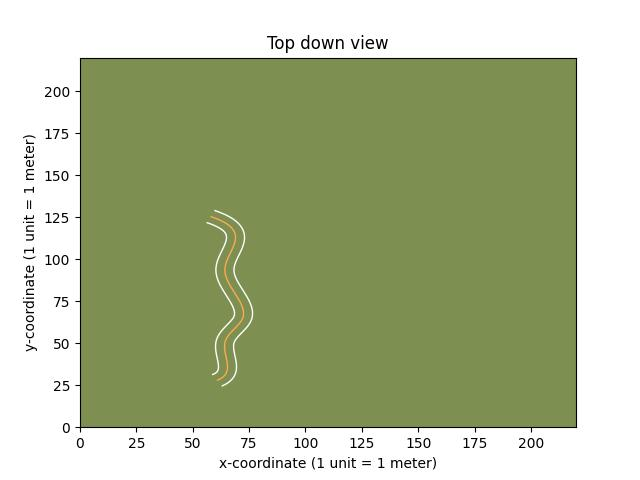
\includegraphics[width=0.5\linewidth]{images/road.jpg}
    \caption{Bird's-Eye View of a road}
    \label{road}
\end{figure}

\begin{figure}[!h]
    \centering
    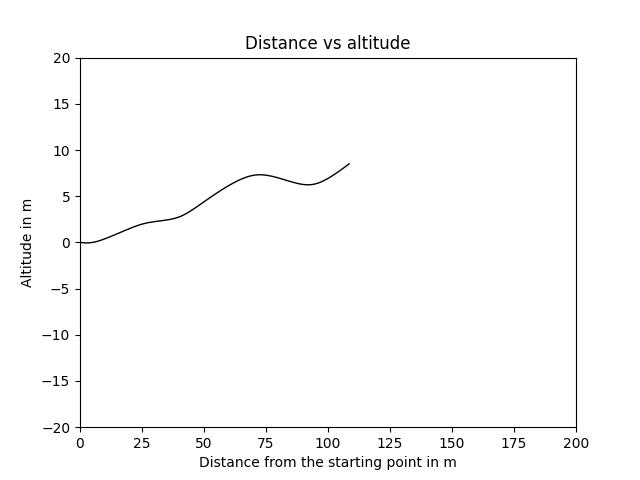
\includegraphics[width=0.5\linewidth]{images/height.jpg}
    \caption{Distance against Height}
    \label{height}
\end{figure}


\chapter{Evaluation}
For the evaluation of the tool, I used the CSV files to analyze the quantitative data produced by the tool. To assess whether the roads generated by ChatGPT align with the description and whether ChatGPT generates diverse roads with the same prompt, I conducted a user study. The results of the data analysis will be described below.

\section{Analysis of the CSV Files}
To analyze generation statistics, three prompts of varying specificity were used: "a road", "an uphill road with 3 turns", and "a road going uphill for 2 turns, followed by a straight downhill segment, ending in a left turn". A combined total of 300 roads were generated, with 100 roads produced for each prompt. Following the simulations, two CSV files were created for each prompt. One contained generation statistics (number of roads generated, valid/invalid counts), while the other recorded instances of cars driving out of their lanes. Of the 300 roads generated, 182 successfully passed validation, with 118 failing. Among the 182 roads simulated, the car steered out of its lane in 8 instances.

Among the 100 roads generated using the prompt "a road," 88 successfully passed validation, and 1 of those 88 roads resulted in the car driving out of the lane. For the prompt "an uphill road with 3 turns," out of the 100 roads generated, 57 met validation criteria, with 2 of those 57 ending with the car steering out of the lane. Lastly, from the 100 roads generated with the prompt "a road going uphill for 2 turns, followed by a straight downhill segment, ending in a left turn," only 37 successfully passed validation, with 5 out of those 37 roads ending with the car driving out of the lane.

This indicates that when prompts are more generic and the language model has more freedom, it tends to better adhere to the specified rules, such as the map size. However, roads generated from more general prompts seem to place less emphasis on testing the lane-keeping functionality of the self-driving agent compared to roads generated from more specific prompts.

The chi-squared test was used to determine the statistical significance of these results. Regarding the number of valid roads generated per prompt, the hypotheses were as follows:

H0: the prompt does not influence the number of valid roads generated
H1: the prompt does influence the number of valid roads generated

An alpha value of 0.05 was chosen.

First, a contingency table (\ref{contingency_validity}) was created to display the counts of valid and invalid roads generated for each prompt. This table was then used to derive the expected values table (\ref{expected_values_validity}), calculated using the formula \(\frac{row\ total * column\ total}{grand\ total}\) for each cell. With these two tables, the chi-square score was computed by applying the formula \(\frac{(observed\ value - calculated\ value)^2}{calculated\ value}\) to each element and summing the results \ref{chi_sq_validity}.

The degrees of freedom are determined by the formula \((number\ of\ rows - 1) * (number\ of\ columns - 1)\). The critical chi-square value can be found in the chi-square distribution table in Appendix \ref{chisq_dist_table}, using the degrees of freedom and the alpha value. Since the calculated chi-square value is 55.35, the critical chi-square value is 5.99, and 55.35 is greater than 5.99, the null hypothesis H0 is rejected. This indicates that the prompt does influence the number of valid roads generated.

In the following tables, the prompt "a road" is referred to as prompt 1, the prompt "an uphill road with 3 turns" is referred to as prompt 2, and the prompt "a road going uphill for 2 turns, followed by a straight downhill segment, ending in a left turn" is referred to as prompt 3.


\begin{table}[H]
    \centering
    \begin{tabular}{|c|c|c|c|} \hline 
         &  valid&  invalid& total\\ \hline 
         prompt 1&  88&  12& 100\\ \hline 
         prompt 2&  57&  43& 100\\ \hline 
         prompt 3&  37&  63& 100\\ \hline 
         total&  182&  118& 300\\ \hline
    \end{tabular}
    \caption{Road Validity Contingency Table}
    \label{contingency_validity}
\end{table}

\begin{table}[H]
    \centering
    \begin{tabular}{|c|c|c|c|} \hline 
         &  valid&  invalid& total\\ \hline 
         prompt 1&  60.67&  39.33& 100\\ \hline 
         prompt 2&  60.67&  39.33& 100\\ \hline 
         prompt 3&  60.67&  39.33& 100\\ \hline 
         total&  182&  118& 300\\ \hline
    \end{tabular}
    \caption{Road Validity Expected Values Table}
    \label{expected_values_validity}
\end{table}

\begin{table}[H]
    \centering
    \begin{tabular}{|c|c|c|c|} \hline 
         &  observed&  calculated& \(\frac{(o-c)^2}{c}\) \\ \hline 
         &  88&  60.67& 12.32\\ \hline 
         &  57&  60.67& 0.22\\ \hline 
         &  37&  60.67& 9.32\\ \hline 
         &  12&  39.33& 18.99\\ \hline 
         &  43&  39.33& 0.34\\ \hline 
         &  63&  39.33& 14.24\\ \hline 
         total&  &  & 55.35\\ \hline
    \end{tabular}
    \caption{Road Validity Chi-Square Calculation}
    \label{chi_sq_validity}
\end{table}

\section{Survey}
For the user study, I distributed a survey to 11 individuals engaged in research or work related to autonomous vehicles. Of these, ten respondents provided answers.

\subsection{Survey structure}
The survey was split into three main sections. The first section aimed to gather demographic information from the participants. The second section asked participants to rate the alignment between a road and the prompt it was generated with. To assist in their evaluation, participants were provided with a bird's-eye view plot, an altitude plot, and two videos depicting a car driving on the road. The first video displayed the car from a third-person perspective, while the second one provided a view from the car's bonnet. In the final section, participants were asked to rate the similarity between two roads generated using the same prompt. For this task, the participants were provided with the altitude plot and the bird's eye view of each road stacked on top of each other, alongside two videos featuring a split-screen view of a car driving on both roads simultaneously. The first split-screen video showed the two cars from a third-person view, while the second one provided a view from the car's bonnets.

Given that all roads used in the user study fall within the coordinate range of 0 to 220, the axes of the bird's-eye view plot are set to span from point 0 to 220, with each unit on the plot representing 1 meter. The axis dimensions were selected to offer a neutral perspective of the roads, avoiding any emphasis on the turns of one road over another. Given that the maximum altitude and longest road length are restricted to 20 and 200 meters, respectively, these factors determine the scaling of the axes for visualizing distance and height in the plot.

\subsection{Survey results}
In this section, I will describe the results of the survey by section.
\subsubsection{Demographic Data}
The participants were asked about their age, occupation, possession of a driver's license, number of countries they have driven in, prior experience with generative AI, and familiarity with driving simulators.

Four participants fall within the age range of 20 to 29 years, five are aged between 30 to 39, and one participant is aged between 40 to 49 (see Figure \ref{age}). Nine participants hold a driver's license, while one does not (see Figure \ref{drivers-license}). Each participant has driven in at least one country (see Figure \ref{countries-driven-in}). Seven participants use generative AI regularly, while three reported using it occasionally (see Figure \ref{genai}). Eight participants use driving simulators regularly, one uses them occasionally, and one participant has never used a driving simulator before (see Figure \ref{driving-simulator}).

\begin{figure}[H]
    \centering
    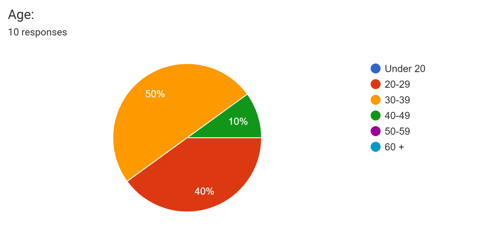
\includegraphics[width=0.6\linewidth]{images/age.png}
    \caption{Age}
    \label{age}
\end{figure}

\begin{figure}[H]
    \centering
    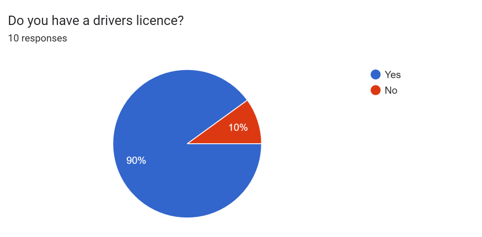
\includegraphics[width=0.5\linewidth]{images/drivers_license.png}
    \caption{Driver's license}
    \label{drivers-license}
\end{figure}

\begin{figure}[H]
    \centering
    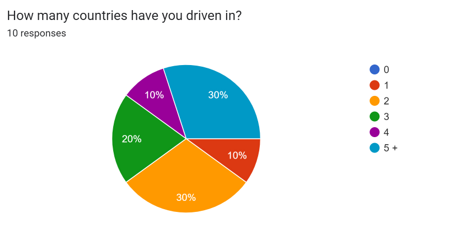
\includegraphics[width=0.6\linewidth]{images/countries_driven_in.png}
    \caption{Countries driven in}
    \label{countries-driven-in}
\end{figure}

\begin{figure}[H]
    \centering
    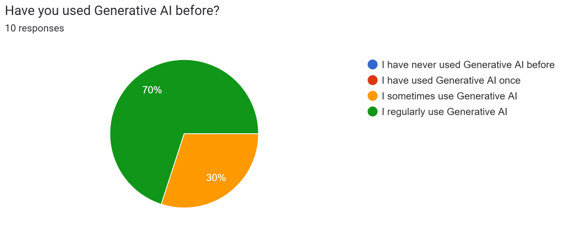
\includegraphics[width=0.7\linewidth]{images/gen_ai.png}
    \caption{Generative AI}
    \label{genai}
\end{figure}

\begin{figure}[H]
    \centering
    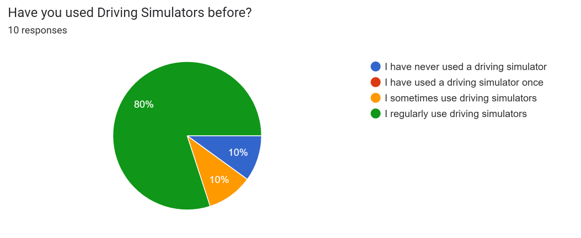
\includegraphics[width=0.7\linewidth]{images/driving_sim.png}
    \caption{Driving Simulator}
    \label{driving-simulator}
\end{figure}

\subsubsection{Road-Prompt Alignment}
In the section concerning Road-Prompt Alignment, participants are tasked with assessing how well a given road corresponds to a provided prompt. This evaluation involves two main components: the overall suitability of the road and its adherence to specific criteria, such as the number of turns, incline, and sequence/order of turns. For visual reference, the participants were presented with an image showing the road plot from both a bird's-eye view and one illustrating altitude side by side as depicted in Figure \ref{road_vis}. Additionally, users had access to two videos: one featuring a car driving on the road from a third-person perspective (see Figure \ref{third-person-view}) and another showing the view from a camera mounted on the car's bonnet (see Figure \ref{bonnet-view}).

\begin{figure}[H]
    \centering
    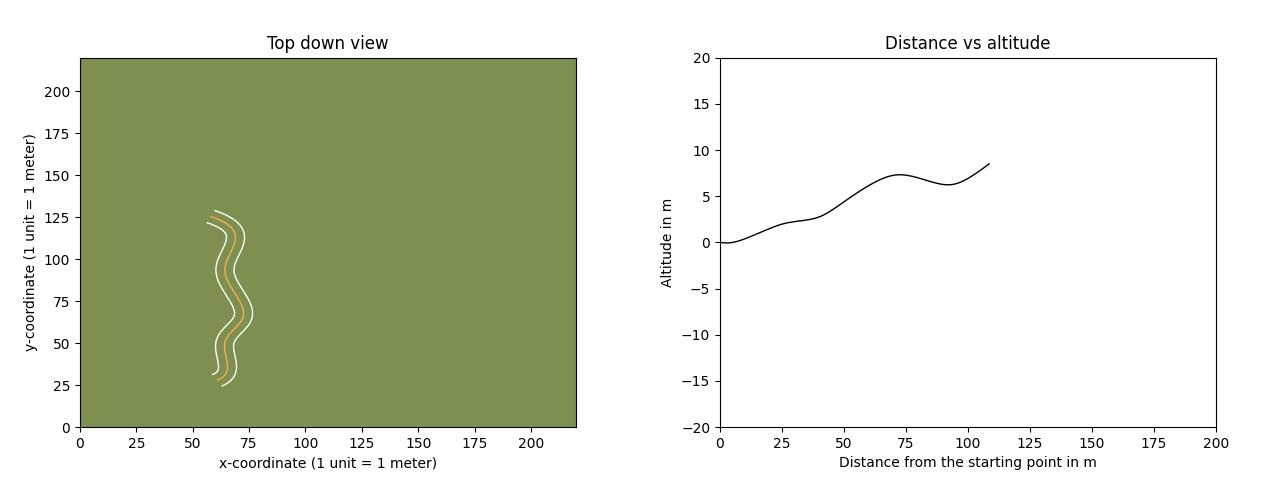
\includegraphics[width=1\linewidth]{images/road3.jpg}
    \caption{Visualization of a road generated with the prompt "a serpentine road"}
    \label{road_vis}
\end{figure}

\begin{figure}[H]
    \centering
    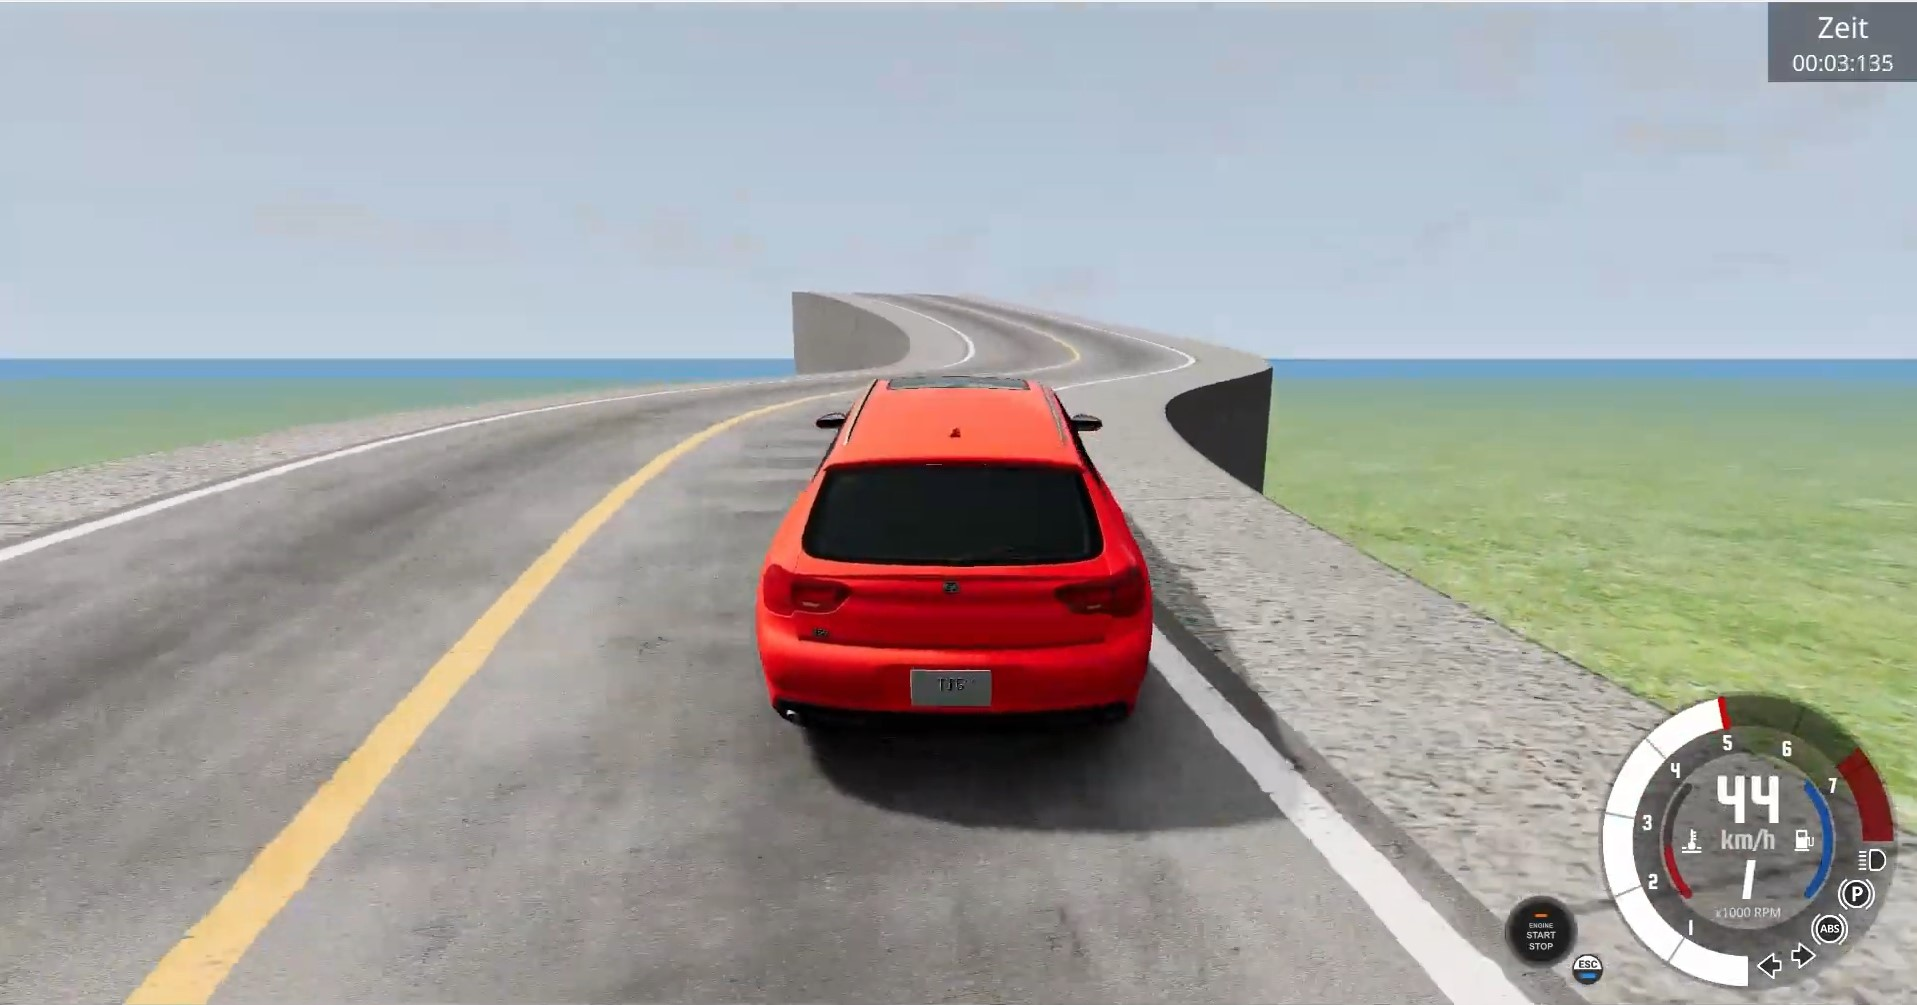
\includegraphics[width=0.5\linewidth]{images/Third_Person_View.jpg}
    \caption{Screenshot from a Video with a Third Person Perspective of a car driving on the road}
    \label{third-person-view}
\end{figure}

\begin{figure}[H]
    \centering
    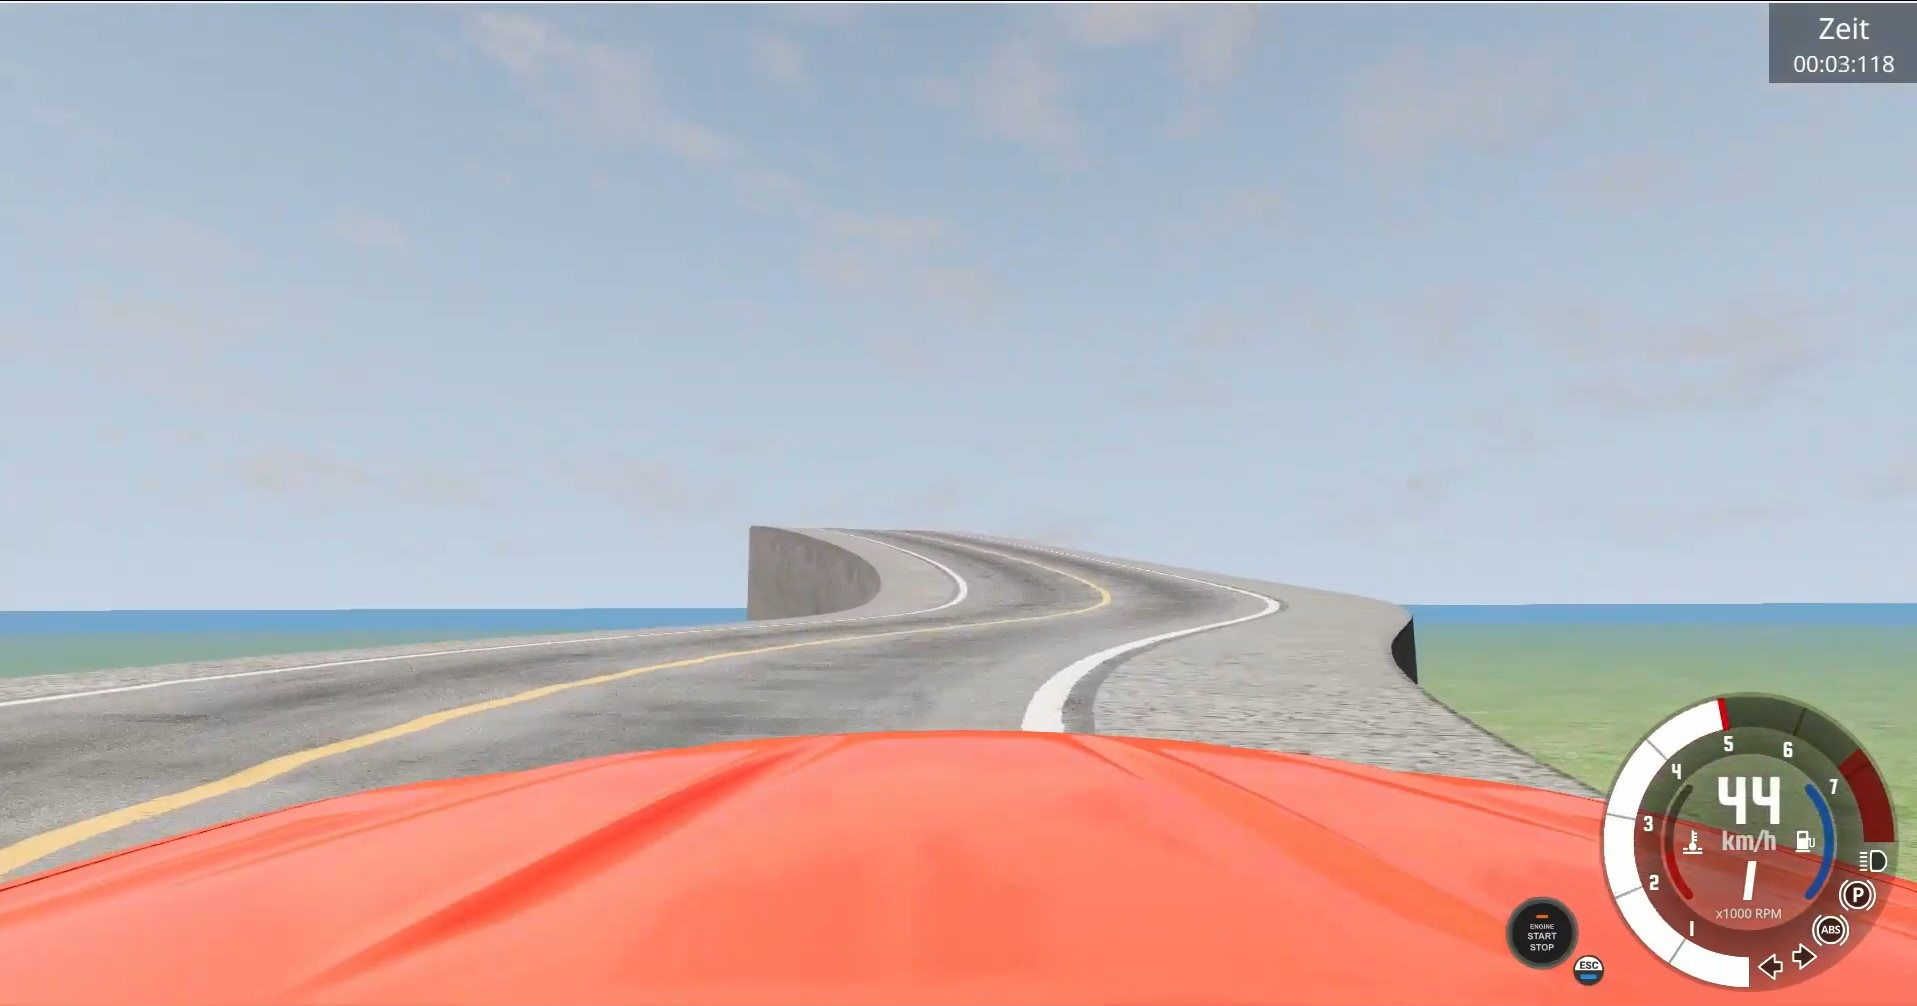
\includegraphics[width=0.5\linewidth]{images/Bonnet_Perspective.jpg}
    \caption{Screenshot from a Video with a Bonnet Perspective of a car driving on the road}
    \label{bonnet-view}
\end{figure}


Four prompts were used for road creation: "a serpentine road", "an uphill road with 3 turns", "a road going uphill for 3 turns and downhill for 2 turns", and "a road going uphill for 2 turns, followed by a straight downhill segment, ending with a left turn." These prompts were chosen to transition from general to more specific. The participants evaluated how well the visualized road matched the respective prompt in both overall fit and specific criteria. Additionally, participants were given the option to provide extra feedback for each road. The participants were required to select from the options "does not match the description at all", "generally does not match the description", "somewhat matches the description", "mostly matches the description", and "perfectly matches the description" in order to cast their votes.

The prompt "a serpentine road" was the most generic prompt used for road generation (see figure \ref{road_vis}). Therefore, participants were only required to rate their overall fit with the prompt. As depicted in figure \ref{serpentine_alignment}, while one participant disagreed, the majority agreed that the road aligned well. Five out of ten participants rated it as a perfect match, one as mostly matching, and three as somewhat matching.

\begin{figure}[H]
    \centering
    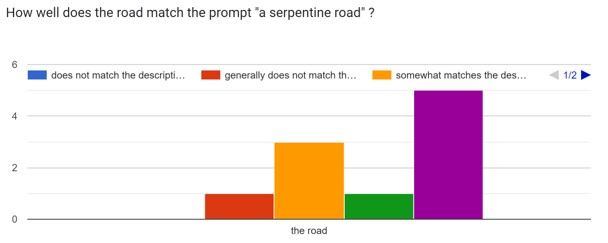
\includegraphics[width=0.75\linewidth]{images/serpentine_general.jpg}
    \caption{Results of the general road-prompt alignment for "a serpentine road"}
    \label{serpentine_alignment}
\end{figure}


The second prompt used was "an uphill road with 3 turns" (see figure \ref{u3t-vis}), which was more detailed as it specified both the incline and the number of turns. Participants indicated that the road generally aligned with the prompt (see figure \ref{u3t-general-alignment}). Regarding the incline, the majority voted that it perfectly matched the prompt, while opinions were divided on the number of turns, with more participants indicating somewhat or mostly matching (see figure \ref{u3t-specific-alignment}). Multiple respondents provided additional feedback, noting a turn starting at the road's end.

\begin{figure}[H]
    \centering
    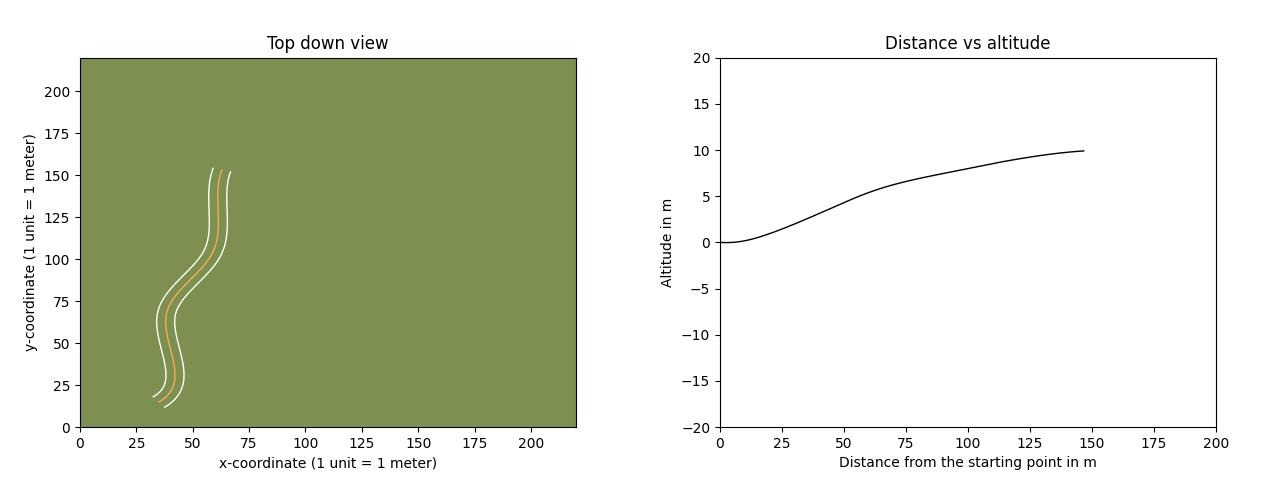
\includegraphics[width=0.75\linewidth]{images/road1.jpg}
    \caption{Visualization of a road generated with the prompt "an uphill road with 3 turns"}
    \label{u3t-vis}
\end{figure}

\begin{figure}[H]
    \centering
    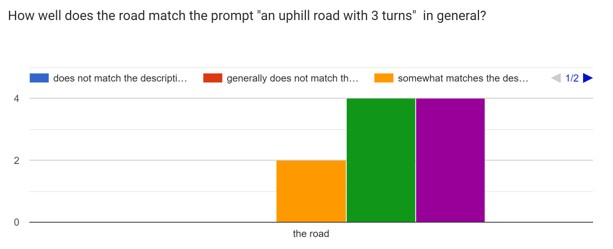
\includegraphics[width=0.75\linewidth]{images/u3t_general.jpg}
    \caption{Results of the general road-prompt alignment for "an uphill road with 3 turns"}
    \label{u3t-general-alignment}
\end{figure}

\begin{figure}[H]
    \centering
    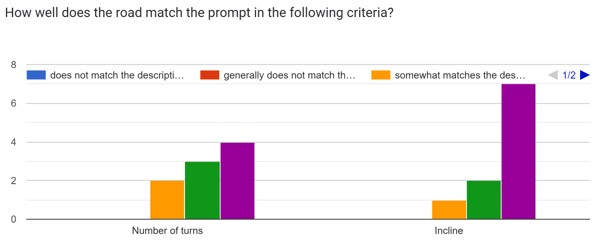
\includegraphics[width=0.75\linewidth]{images/u3t_criteria.jpg}
    \caption{Results of the road-prompt alignment in specific criteria for "an uphill road with 3 turns"}
    \label{u3t-specific-alignment}
\end{figure}

The prompt "a road going uphill for 3 turns and downhill for 2 turns" (see figure \ref{u3t-d2t-vis}) introduced an additional level of specificity by incorporating changes in incline. Although participants generally agreed that the road aligned with the prompt (see figure \ref{u3t-d2t-general}, closer inspection of specific aspects revealed mismatches. While the incline and the number of uphill turns closely matched the prompt, the count of downhill turns did not (figure \ref{u3t-d2t-specific}). In the additional feedback, several participants highlighted the absence of a downhill turn. One participant noted that while the LLM interprets the incline correctly, "counting" the turns does not seem to be a task that it performs well in.

\begin{figure}[H]
    \centering
    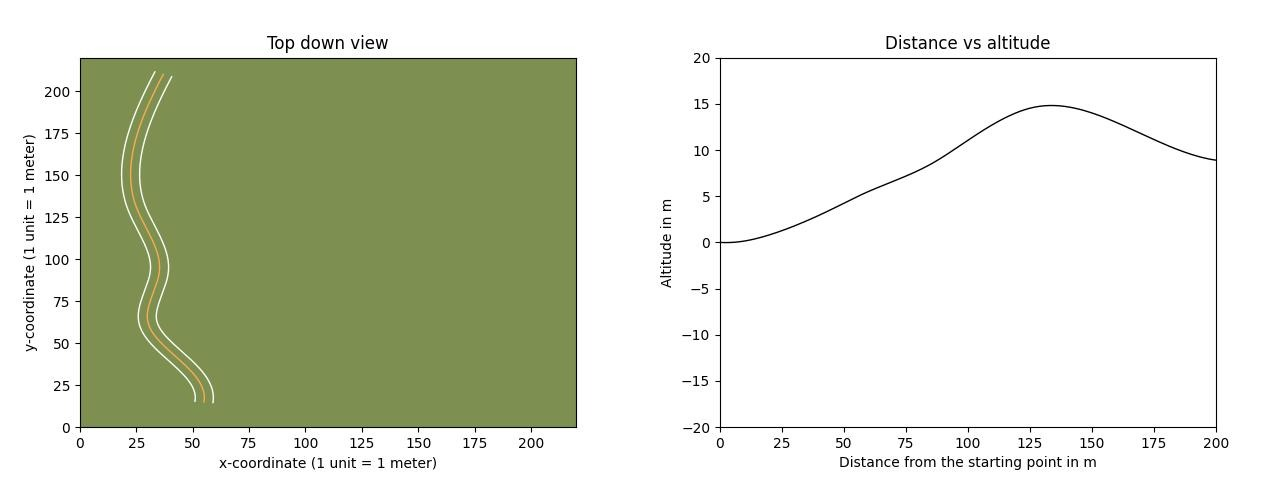
\includegraphics[width=0.75\linewidth]{images/u3t_d2t_vis.jpg}
    \caption{Visualization of a road generated with the prompt "a road going uphill for 3 turns and downhill for 2 turns"}
    \label{u3t-d2t-vis}
\end{figure}

\begin{figure}[H]
    \centering
    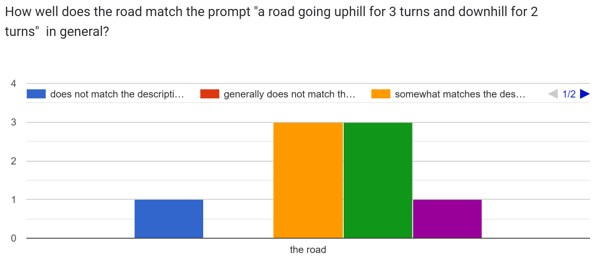
\includegraphics[width=0.75\linewidth]{images/u3t_d2t_general.jpg}
    \caption{Results of the general road-prompt alignment for "a road going uphill for 3 turns and downhill for 2 turns"}
    \label{u3t-d2t-general}
\end{figure}

\begin{figure}[H]
    \centering
    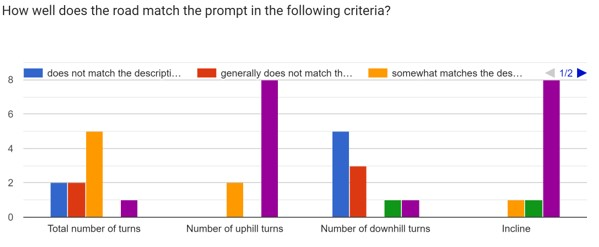
\includegraphics[width=0.75\linewidth]{images/u3t_d2t_specific.jpg}
    \caption{Results of the road-prompt alignment in specific criteria for "a road going uphill for 3 turns and downhill for 2 turns"}
    \label{u3t-d2t-specific}
\end{figure}

The most detailed prompt used is "a road going uphill for 2 turns, followed by a straight downhill segment, ending in a left turn" (figure \ref{most-specific-vis}). The prompt introduces a sequence for the road segments. Although most participants agreed that the road matched the prompt (figure \ref{most-specific-general}), some were unsure about the total number of turns \ref{most-specific-specific-criteria}. In additional comments, two participants mentioned the difficulty in determining whether there was only one turn or two in the uphill segments. Meanwhile, one participant expressed uncertainty about the presence of an additional turn in the uphill segment.

\begin{figure}[H]
    \centering
    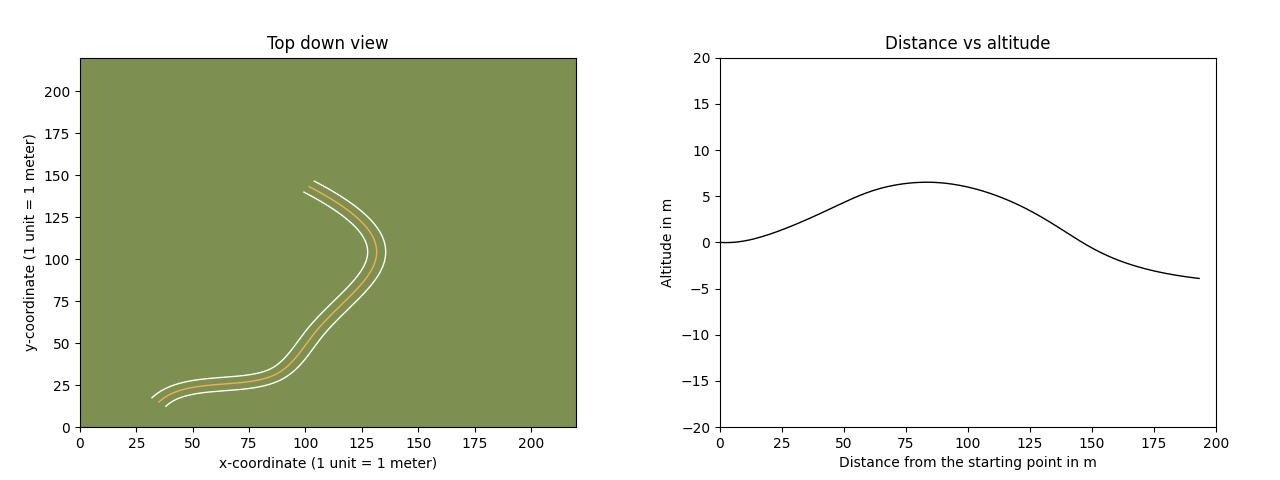
\includegraphics[width=0.75\linewidth]{images/road_height.jpg}
    \caption{Visualization of a road generated with the prompt "a road going uphill for 2 turns, followed by a straight downhill segment, ending in a left turn"}
    \label{most-specific-vis}
\end{figure}

\begin{figure}[H]
    \centering
    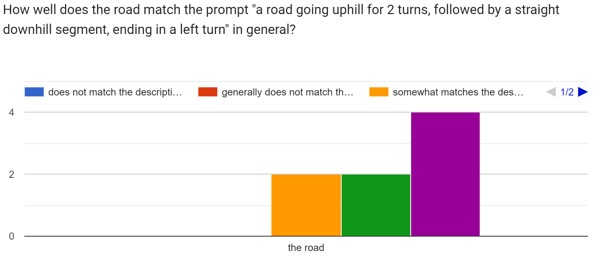
\includegraphics[width=0.75\linewidth]{images/most_specific_general.jpg}
    \caption{Results of the general road-prompt alignment for "a road going uphill for 2 turns, followed by a straight downhill segment, ending in a left turn"}
    \label{most-specific-general}
\end{figure}

\begin{figure}[H]
    \centering
    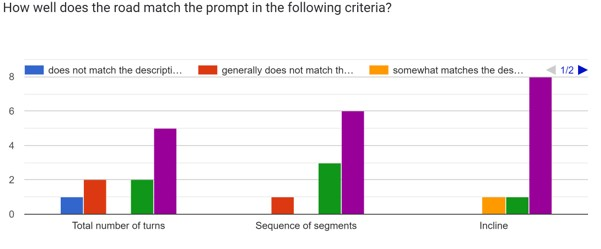
\includegraphics[width=0.75\linewidth]{images/most_specific_specific.jpg}
    \caption{Results of the road-prompt alignment in specific criteria for "a road going uphill for 2 turns, followed by a straight downhill segment, ending in a left turn"}
    \label{most-specific-specific-criteria}
\end{figure}


Reviewing the results, it seems that, as one user pointed out, the LLM performs well at interpreting the incline of the prompts but struggles with accurately identifying the specified number of turns.

\subsubsection{Road Similarity}
In the Road Similarity section, participants were presented with pairs of roads to evaluate their resemblance to each other. Visualizations presented both road plots, one above the other, as shown in figure \ref{comparison_u3t}. Additionally, participants were shown split-screen videos featuring cars driving along both roads simultaneously, with one providing a third-person perspective (figure \ref{splitscreen-tp}) and the other showing the car's perspective from the bonnet (figure \ref{splitscreen-bonnet}). Participants were then prompted to rate the general similarity between the roads and their similarity in specific criteria. Ratings ranged from "definitely different" to "basically the same road" for general similarity and from "definitely different" to "(almost) identical" for specific criteria.

\begin{figure}[H]
    \centering
    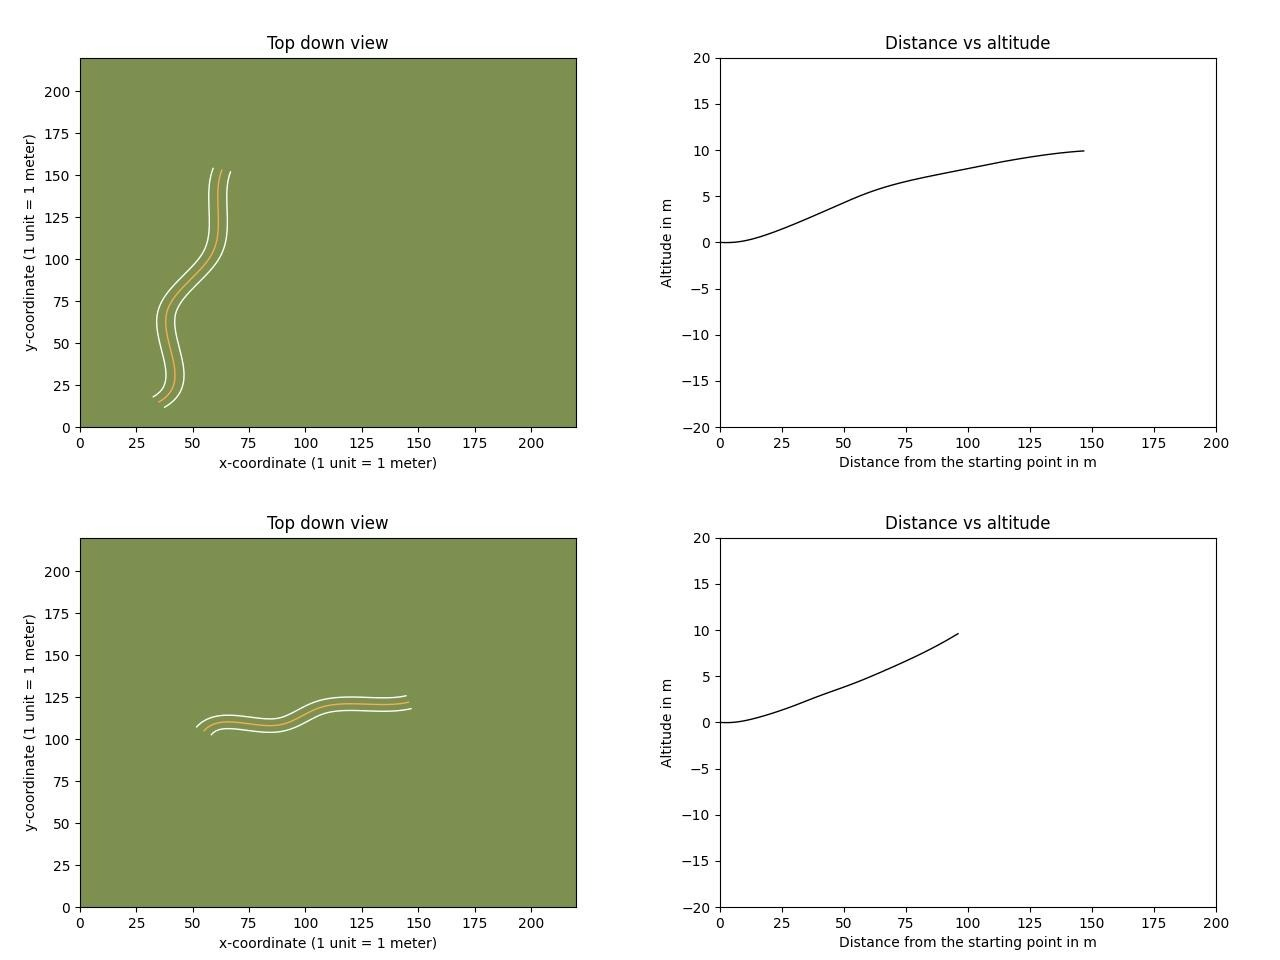
\includegraphics[width=0.75\linewidth]{images/road1_road2.jpg}
    \caption{Comparison of 2 roads generated with the prompt "an uphill road with 3 turns"}
    \label{comparison_u3t}
\end{figure}

\begin{figure}[H]
    \centering
    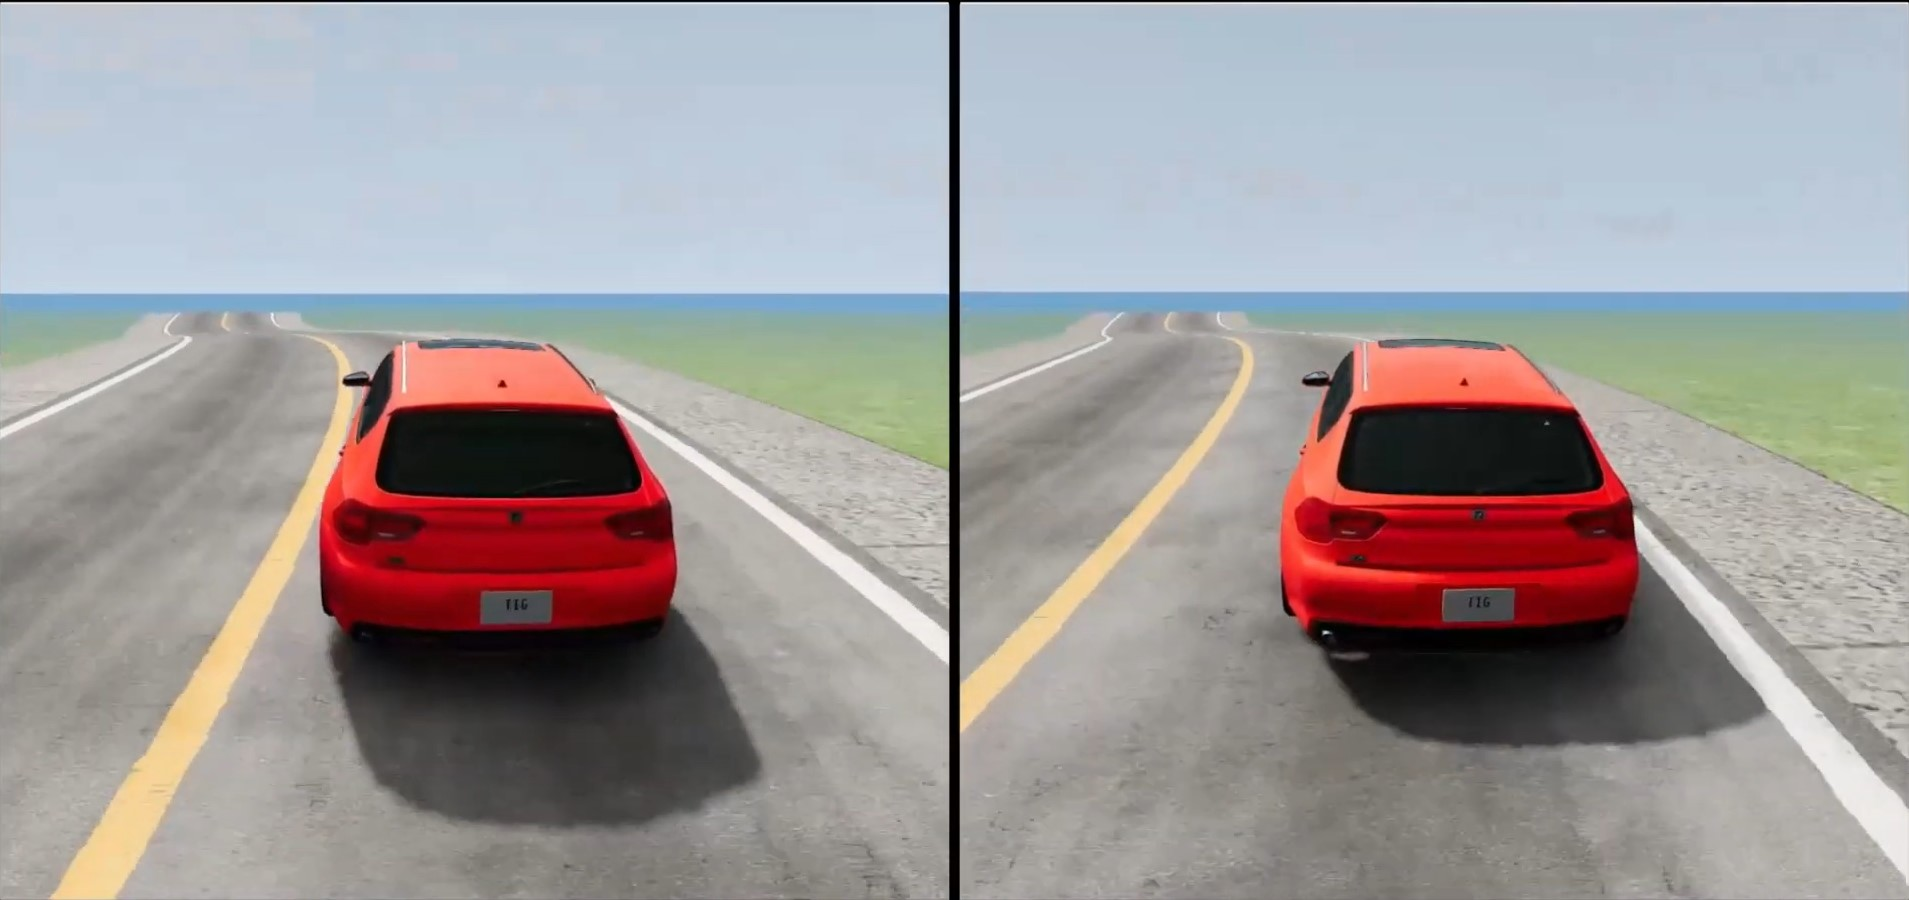
\includegraphics[width=0.75\linewidth]{images/splitscreen_tp_view.jpg}
    \caption{Screenshot from a Split-Screen Video with a Third Person Perspective}
    \label{splitscreen-tp}
\end{figure}

\begin{figure}[H]
    \centering
    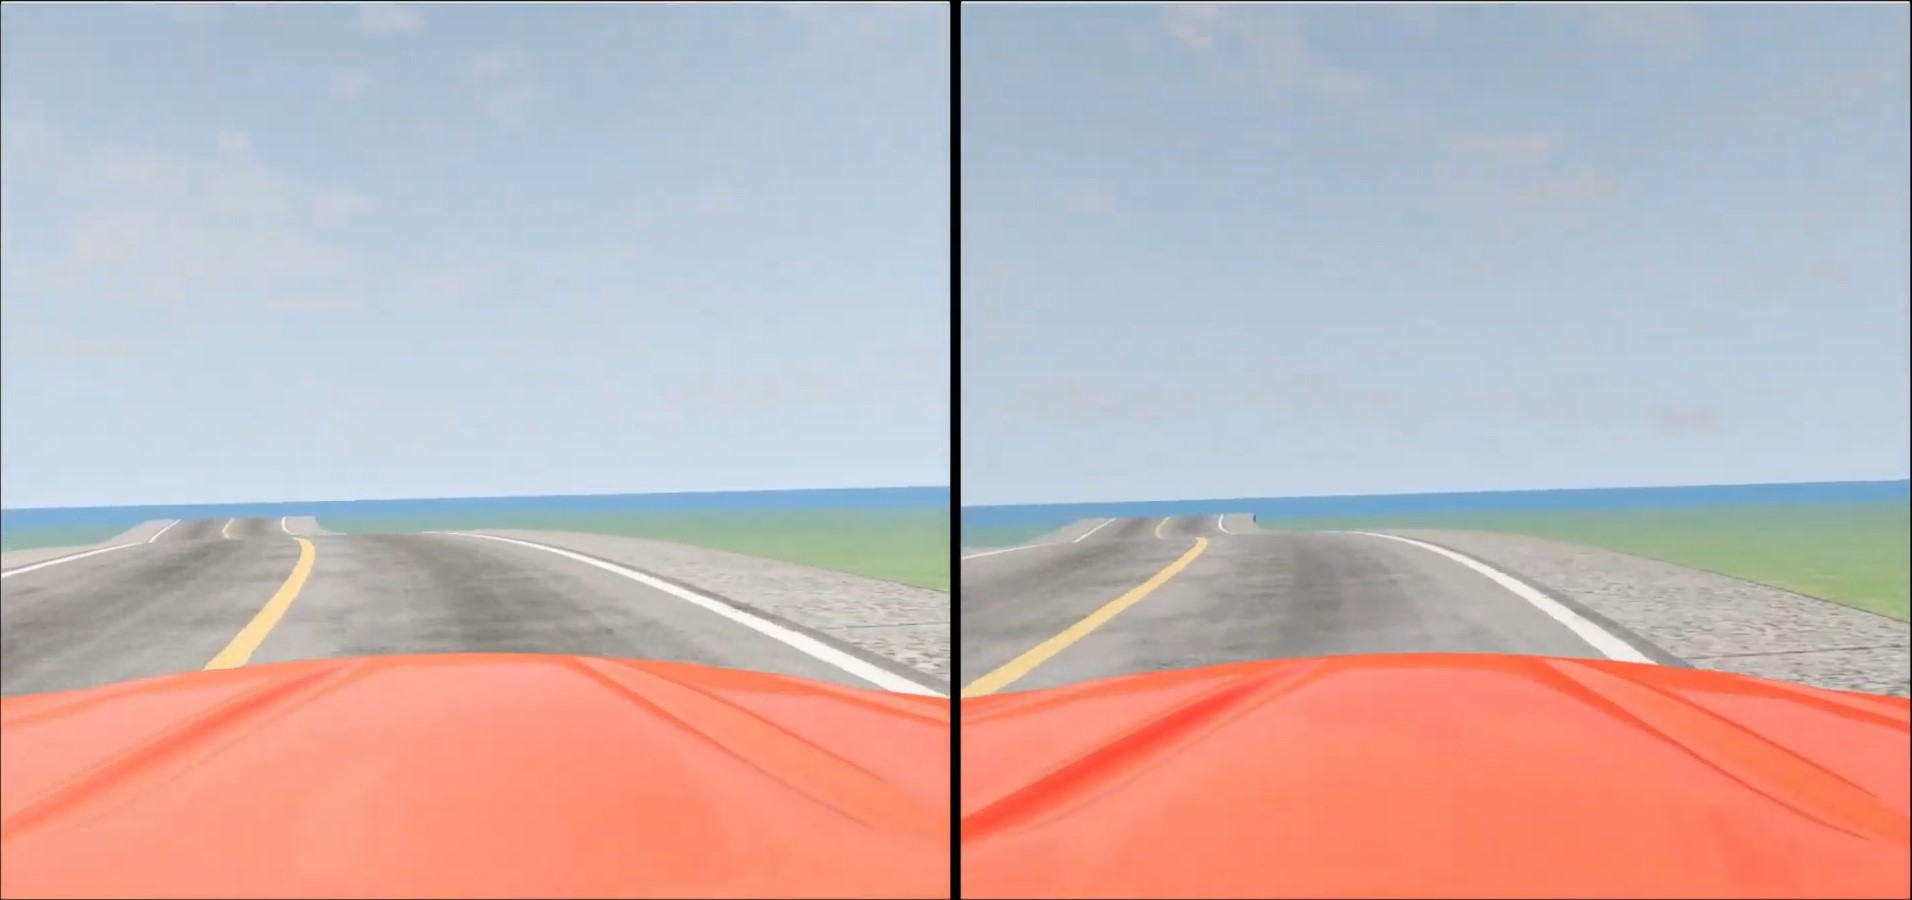
\includegraphics[width=0.75\linewidth]{images/splitscreen_bonnet_view.jpg}
    \caption{Screenshot from a Split-Screen Video with a Bonnet Perspective}
    \label{splitscreen-bonnet}
\end{figure}


The participants generally found the first two roads (figure \ref{comparison_u3t}), which were generated with the prompt "an uphill road with 3 turns",  to be dissimilar, as illustrated in Figure \ref{general_similarity_uphill_road}. Although there was agreement on the similarity in the number of turns, differences were noted in the sequence of turns and the length of the road, which were distinctly perceived as dissimilar. Opinions on the road's incline varied, with three participants rating it as identical while another three rated it as mostly dissimilar (see figure \ref{specific_similarity_uphill_road}).


\begin{figure}[H]
    \centering
    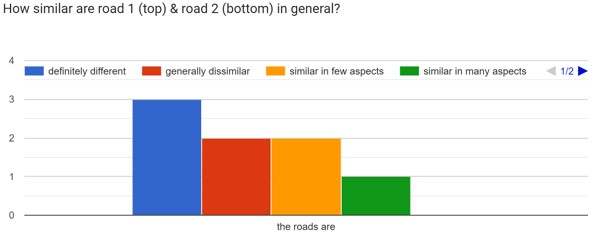
\includegraphics[width=0.75\linewidth]{images/similarity_a_road.jpg}
    \caption{General similarity of the two roads generated with the prompt "an uphill road with 3 turns"}
    \label{general_similarity_uphill_road}
\end{figure}

\begin{figure}[H]
    \centering
    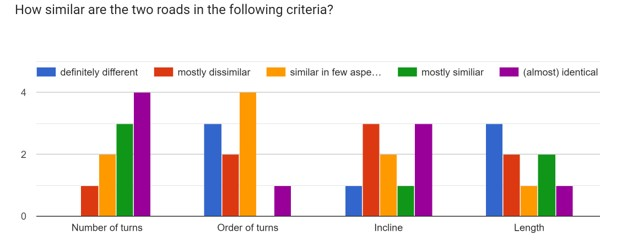
\includegraphics[width=0.75\linewidth]{images/similarity_a_road_specific.jpg}
    \caption{Similarity in certain criteria of the two roads generated with the prompt "an uphill road with 3 turns"}
    \label{specific_similarity_uphill_road}
\end{figure}


The second pair of roads, generated with the prompt "a road" (figure \ref{comparison_a_road}), were perceived as identical (figure \ref{general_similarity_a_road}). Participants rated the roads as identical across all criteria (figure \ref{specific_similarity_a_road}). Several participants noted in the additional comments that the only difference was the orientation of the roads in the bird's eye view plot.


\begin{figure}[H]
    \centering
    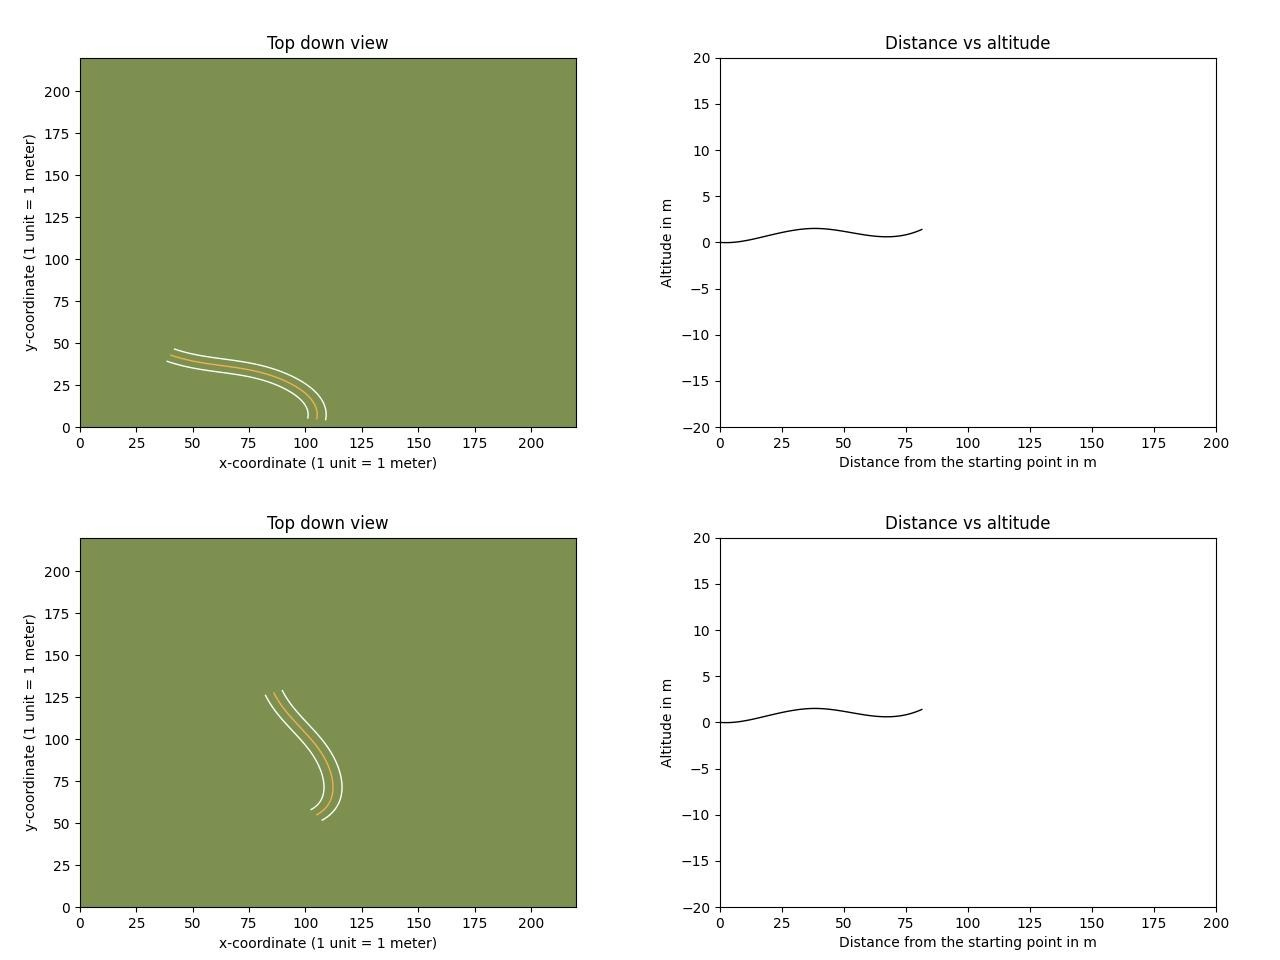
\includegraphics[width=0.75\linewidth]{images/road2_road3.jpg}
    \caption{Comparison of 2 roads generated with the prompt "a road"}
    \label{comparison_a_road}
\end{figure}

\begin{figure}[H]
    \centering
    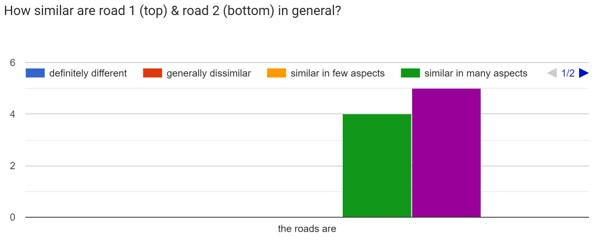
\includegraphics[width=0.75\linewidth]{images/similarity2_general.jpg}
    \caption{General similarity of the two roads generated with the prompt "a road"}
    \label{general_similarity_a_road}
\end{figure}

\begin{figure}[H]
    \centering
    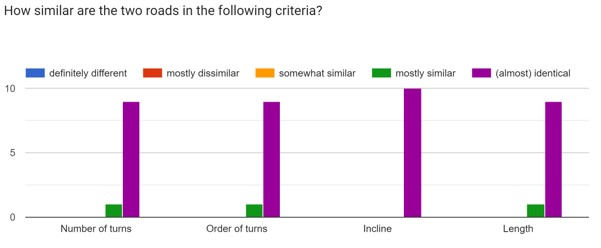
\includegraphics[width=0.75\linewidth]{images/similarity2_specific.jpg}
    \caption{Similarity in certain criteria of the two roads generated with the prompt "a road"}
    \label{specific_similarity_a_road}
\end{figure}

In conclusion, the LLM is proficient in generating roads that meet specific criteria outlined in the prompts. While it accurately interprets inclines, determining the number of turns remains a challenge. When presented with identical prompts, ChatGPT sometimes produces roads that are almost identical, with the main difference being their orientation.


\section{Conclusion}

This section summarizes the results to address the research question \textbf{Can generative AI be used to automatically create three-dimensional roads for testing autonomous vehicles?}

The results imply that Generative AI has the potential to create virtual roads that are appropriate for testing autonomous vehicles. ChatGPT was used due to its accessibility and seamless integration via the OpenAI API. Despite the model not being trained for this particular use case, it produced roads that met most requirements. The user study indicated that while ChatGPT performed well in interpreting road inclines, it struggled with generating the correct number of turns and stressing the lane-keeping functionality of the self-driving agent. Since the model is not specifically trained or designed for this task, potential solutions to these issues may include the creation of a labeled dataset for fine-tuning or the training of a new model.

\section{Open Issues and Possible Improvements}

The evaluation of the tool revealed several issues. Firstly, it was found that the more specific the prompt, the fewer roads passed validation checks. Secondly, the generated roads lack scenarios that effectively challenge the lane-keeping functionality of autonomous vehicles. Additionally, ChatGPT struggled to generate the correct number of turns accurately. As ChatGPT is not explicitly trained for road generation, these issues might be resolved by compiling a labeled dataset with road descriptions as labels and the anticipated LLM output for fine-tuning an existing model, or by training a new model altogether. 

A participant in the user study pointed out that \textit{It would match better with the prompt if the generated road had straight segments at the start and end (which can be part of the prompt), so the number of turns was more obvious. Now, the road starts in the middle of the turn, and it has a small turn at the end of the road, too.} This feedback should be considered for future work stemming from this project.
\chapter{Summary}

The objective of this thesis was to create a tool utilizing generative AI to generate virtual roads for testing self-driving vehicles. The system was designed to streamline the process of testing autonomous vehicles by converting textual road descriptions into coordinate-based nodes. These nodes are used to construct the road within the simulation environment. This approach eliminates the need to write complicated algorithms.

The tool's implementation involved selecting appropriate technologies, such as the programming language, the chosen LLM, and the simulator. The evaluation comprised a quantitative analysis of the number of generated roads and instances where the car deviated from its lane, alongside a survey gathering feedback from target users regarding the generated roads.

Although the model didn't effectively stress the lane-keeping functionality, it's important to note that it wasn't trained for that purpose. Nevertheless, the model generally produced roads that aligned with the provided descriptions.

In conclusion, the tool developed in this thesis presents a promising solution for generating virtual roads using generative AI. The study results suggest that the tool holds the potential to serve as a foundation for future research in this field.


\section{Future work}

While this study established the groundwork for using generative AI in road generation, there are still many areas to explore to enhance the performance of AI models in this task.

\textbf{Fine-Tuning a model}: By compiling a dataset containing road descriptions paired with descriptive prompts as labels, it is possible to fine-tune a model specifically for this purpose and enhancing its performance. This dataset can be constructed either by labeling roads generated by an existing tool or by manually generating roads based on provided prompts.

\textbf{Training a new model}: Training a new model allows for fine-tuning it for specific purposes, ensuring adherence to all relevant rules. This can be achieved by training the model on either artificially generated roads or real roads. While training on generated roads can effectively stress test the lane-keeping functionality of the self-driving agent, training on real-world roads ensures that the model closely mimics real-world scenarios.

\textbf{Terrain modification}: At the time of writing, BeamNgpy introduced new functionality allowing users to import heightmaps and enable terrain modification. This introduces a challenge as road sections might be obscured by terrain. Moreover, when combined with traffic, it not only tests the car's lane-keeping capabilities but also its ability to avoid collisions. 

\textbf{Road Networks}: Expanding the functionality of road generation tools to encompass entire road networks, including features such as junctions, offers numerous advantages. It provides a more comprehensive evaluation of autonomous vehicles in varied driving environments, testing their ability to navigate complex intersections and merge lanes. Including diverse lane markings enhances realism, resulting in more precise performance evaluations and better preparation for real-world deployment. In essence, shifting from individual roads to complete road networks enhances testing precision and helps in the development of safer autonomous driving systems.


%   BACK MATTER  %%%%%%%%%%%%%%%%%%%%%%%%%%%%%%%%%%%%%%%%%%%%%%%%%%%%%%%%%%%%%%
%
%   References and appendices. Appendices come after the bibliography and
%   should be in the order that they are referred to in the text.
%
%   If you include figures, etc. in an appendix, be sure to use
%
%       \caption[]{...}
%
%   to make sure they are not listed in the List of Figures.
%

\backmatter%
	\addtoToC{Bibliography}
	\bibliographystyle{IEEEtranS}
 \typeout{}
	\bibliography{references}
	

\begin{appendices} % optional
\chapter{Example Appendix 1}

\begin{table}
    \centering
    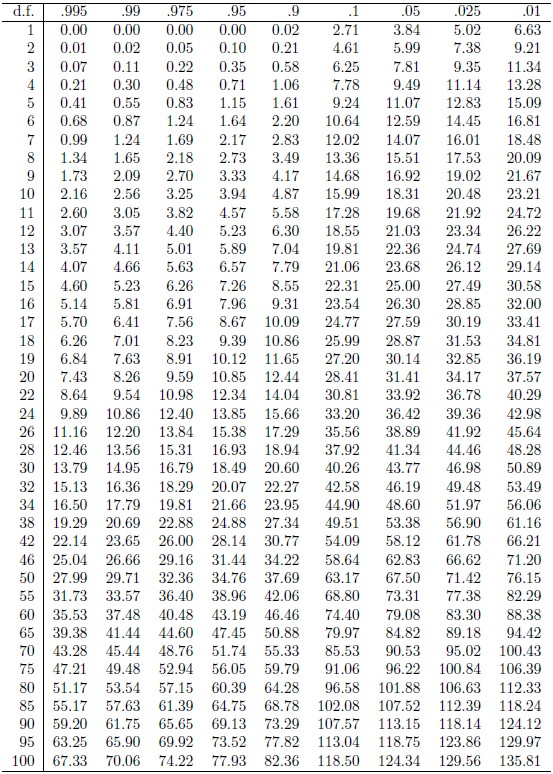
\includegraphics[width=1\linewidth]{chisq.jpg}
    \caption{Chi-Square Distribution Table. Adapted from \cite{Freedman_2007}}
    \label{chisq_dist_table}
\end{table}

%Appendices should be used for supplemental information that does not form part of the main research. Remember that figures and tables in appendices should not be listed in the List of Figures or List of Tables. 

%\chapter{Example Appendix 2}

%Appendices should be used for supplemental information that does not form part of the main research. Remember that figures and tables in appendices should not be listed in the List of Figures or List of Tables. 
	
\end{appendices}
\end{document}
